\chapter{Distribution of input features to the \ggH and VBF BDTs}
\label{app:all_input_features}

%%%ggH%%%

The distribution of each input feature to the \ggH BDT is shown in Figures \ref{fig:ggH_inputs_first}--\ref{fig:ggH_inputs_last} for the DY and \ttbar backgrounds, data, 
and \ggH signal. The agreement between data and simulated background events is reasonable; however, any non-closure cannot bias the modelling of background events in the final fit. Similarly, Figures \ref{fig:VBF_inputs_first}--\ref{fig:VBF_inputs_last} show inputs to the VBF BDT for simulated DY, \ttbar, and electroweak Z boson background processes, data, and VBF signal. Agreement between data and simulated background events is good.

\begin{figure}[htbp!]
\centering
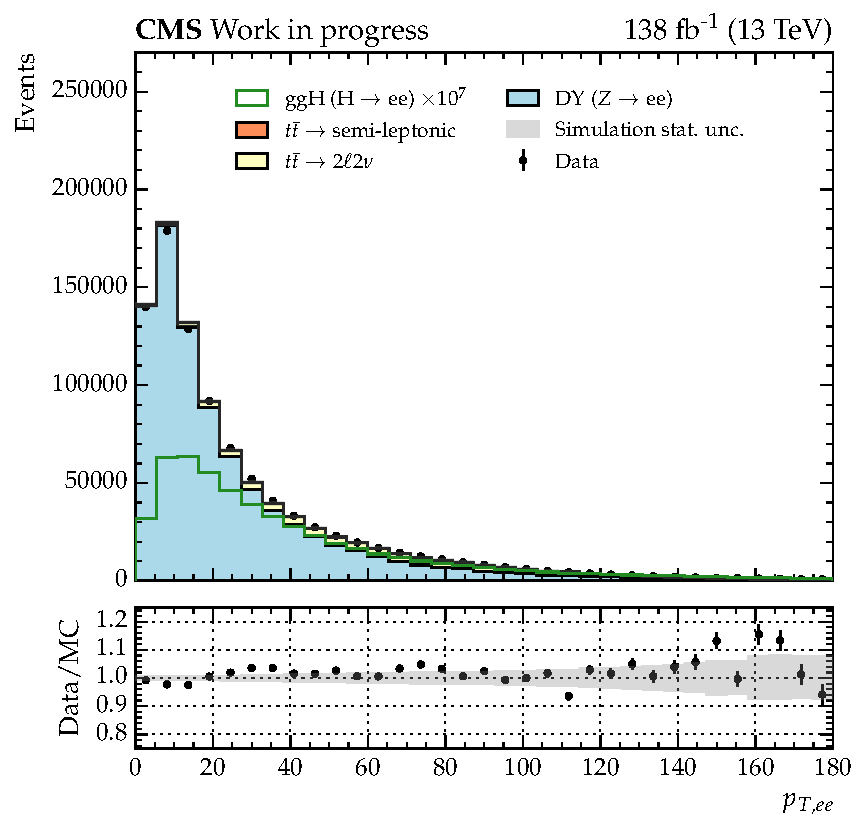
\includegraphics[width =0.33\linewidth]{Figures/Hee/ggH/dataMC/all_inputs/ggH_BDT_pt_reweighted_dielectronPt.pdf}\hfill%
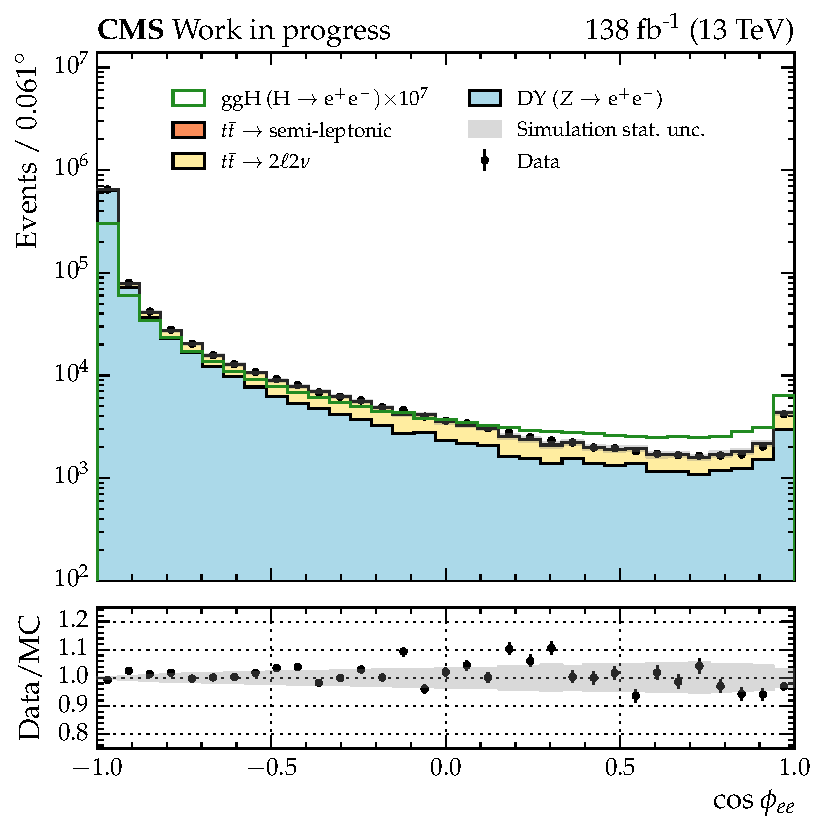
\includegraphics[width =0.32\linewidth]{Figures/Hee/ggH/dataMC/all_inputs/ggH_BDT_pt_reweighted_dielectronCosPhi.pdf}\hfill%
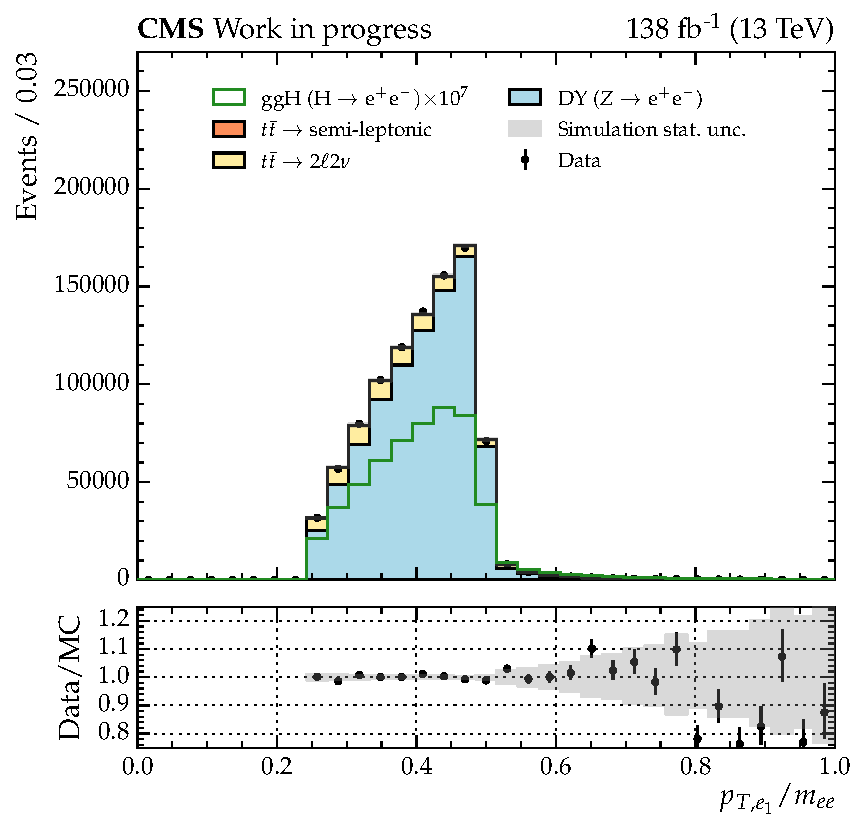
\includegraphics[width =0.33\linewidth]{Figures/Hee/ggH/dataMC/all_inputs/ggH_BDT_pt_reweighted_subleadElectronPtOvM.pdf}\hfill%
 
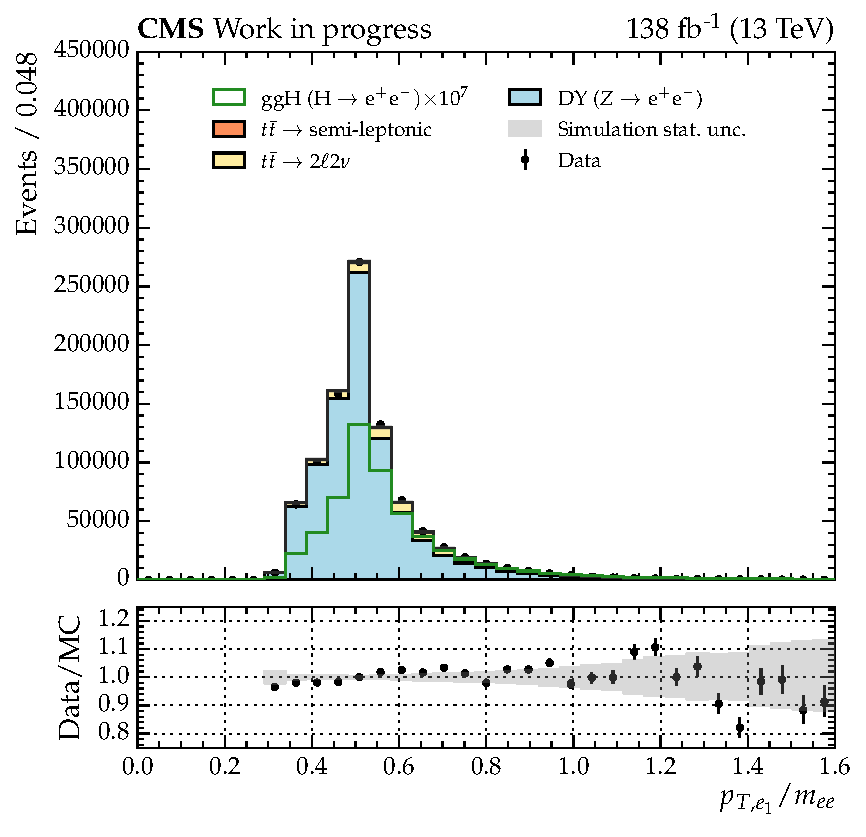
\includegraphics[width =0.33\linewidth]{Figures/Hee/ggH/dataMC/all_inputs/ggH_BDT_pt_reweighted_leadElectronPtOvM.pdf}\hfill%
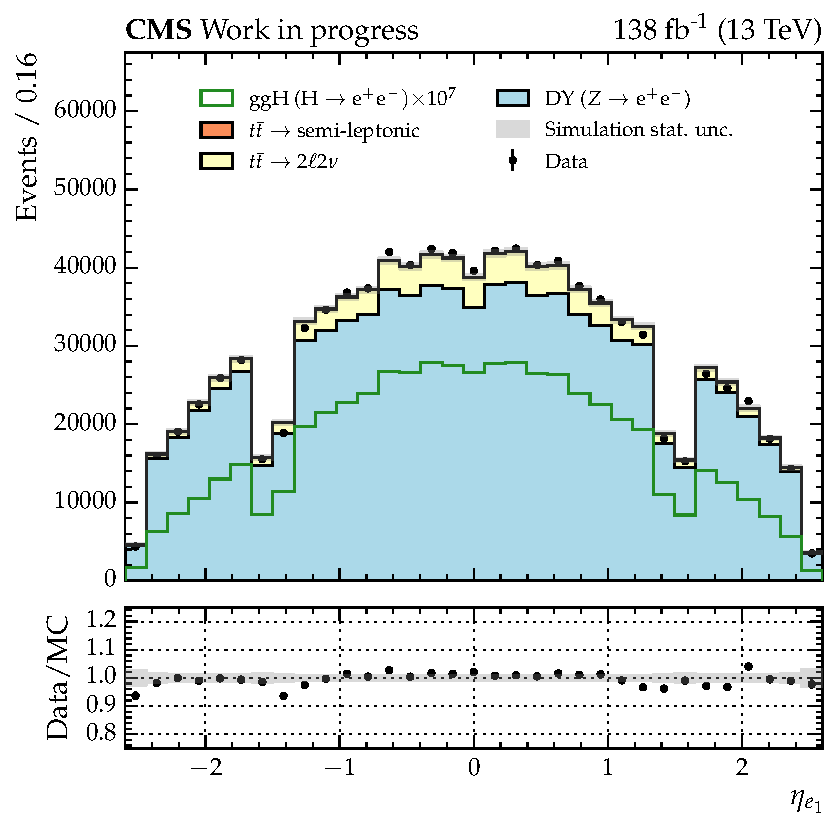
\includegraphics[width =0.33\linewidth]{Figures/Hee/ggH/dataMC/all_inputs/ggH_BDT_pt_reweighted_leadElectronEta.pdf}\hfill%
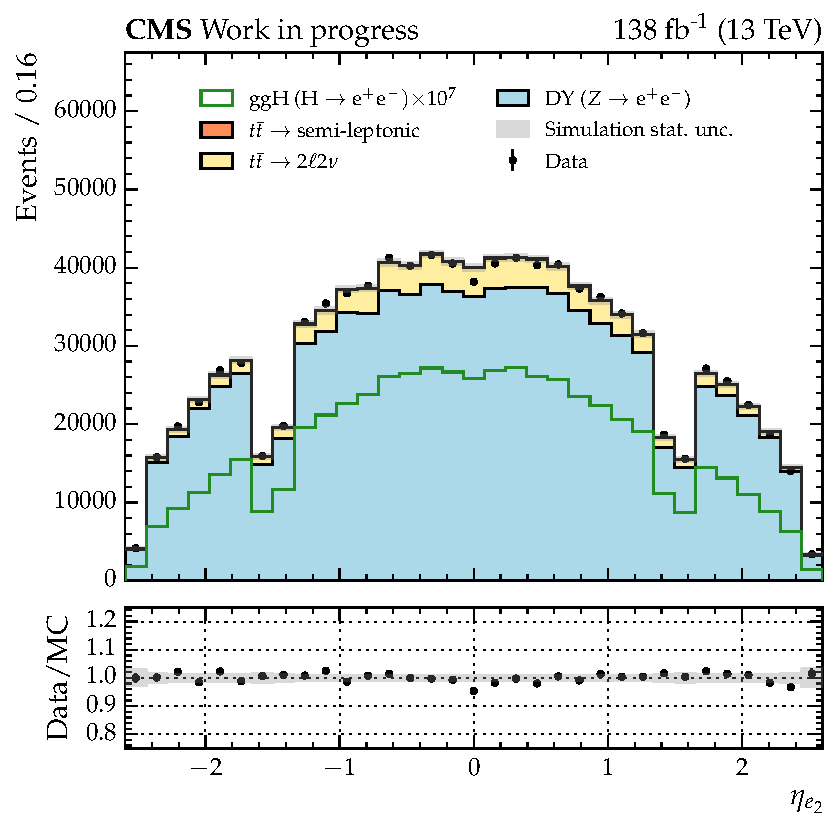
\includegraphics[width =0.33\linewidth]{Figures/Hee/ggH/dataMC/all_inputs/ggH_BDT_pt_reweighted_subleadElectronEta.pdf}\hfill%
 
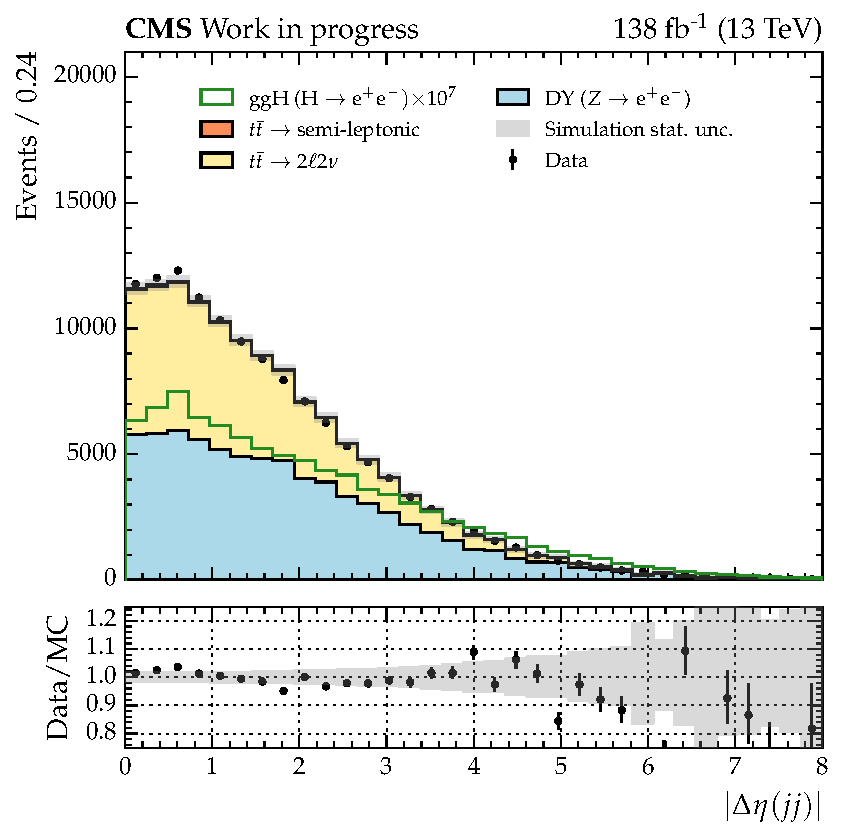
\includegraphics[width =0.33\linewidth]{Figures/Hee/ggH/dataMC/all_inputs/ggH_BDT_pt_reweighted_dijetAbsDEta.pdf}\hfill%
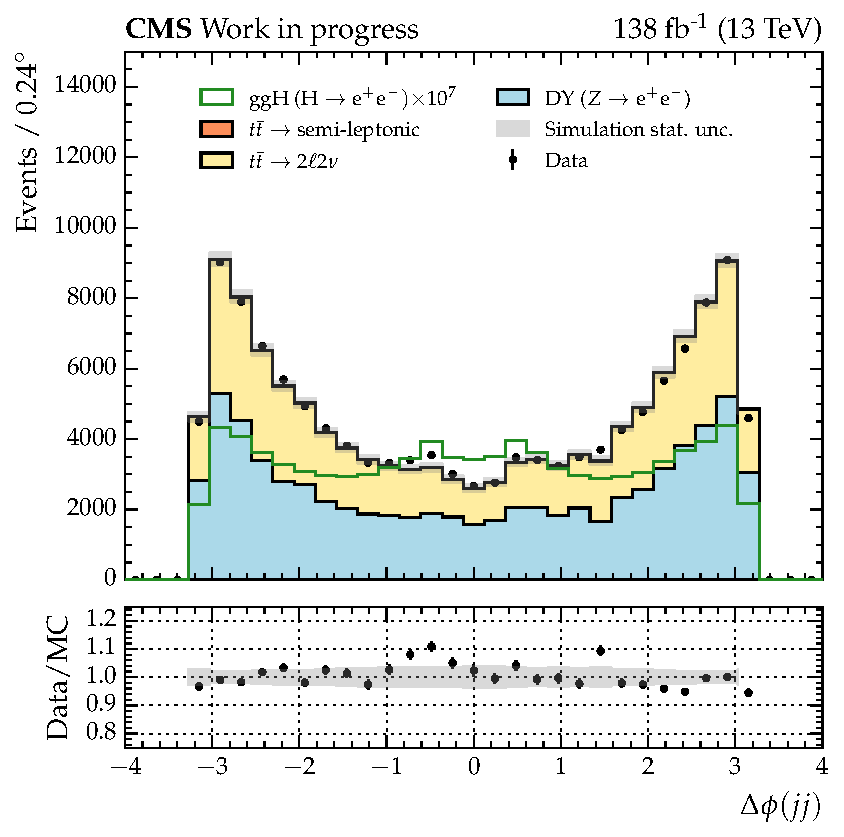
\includegraphics[width =0.33\linewidth]{Figures/Hee/ggH/dataMC/all_inputs/ggH_BDT_pt_reweighted_dijetDPhi.pdf}\hfill%
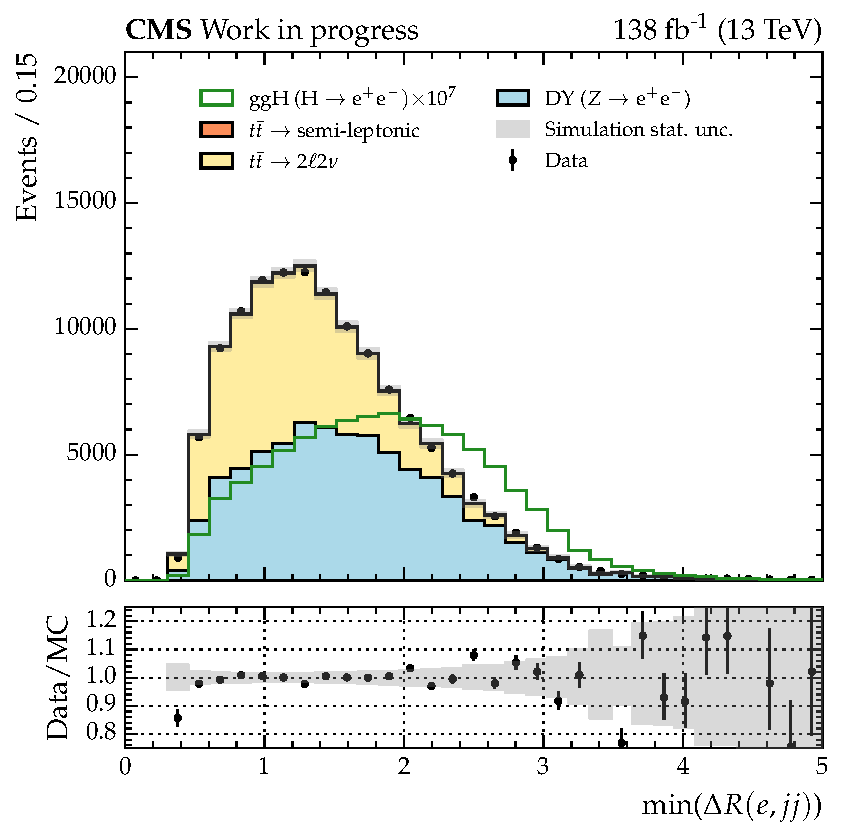
\includegraphics[width =0.33\linewidth]{Figures/Hee/ggH/dataMC/all_inputs/ggH_BDT_pt_reweighted_dijetMinDRJetEle.pdf}\hfill%
 
\caption{Distributions for the input variables to the gluon-fusion BDT. The ggH signal is shown in green, with the overall normalisation scaled such that it is visible. The simulated background processes (bold face) are stacked for comparison with data (black points). Reasonable agreement is observed between data and simulation, with respect to the statistical uncertainty (grey band).}
\label{fig:ggH_inputs_first}
\end{figure}
 
\begin{figure}[htbp!]
\centering
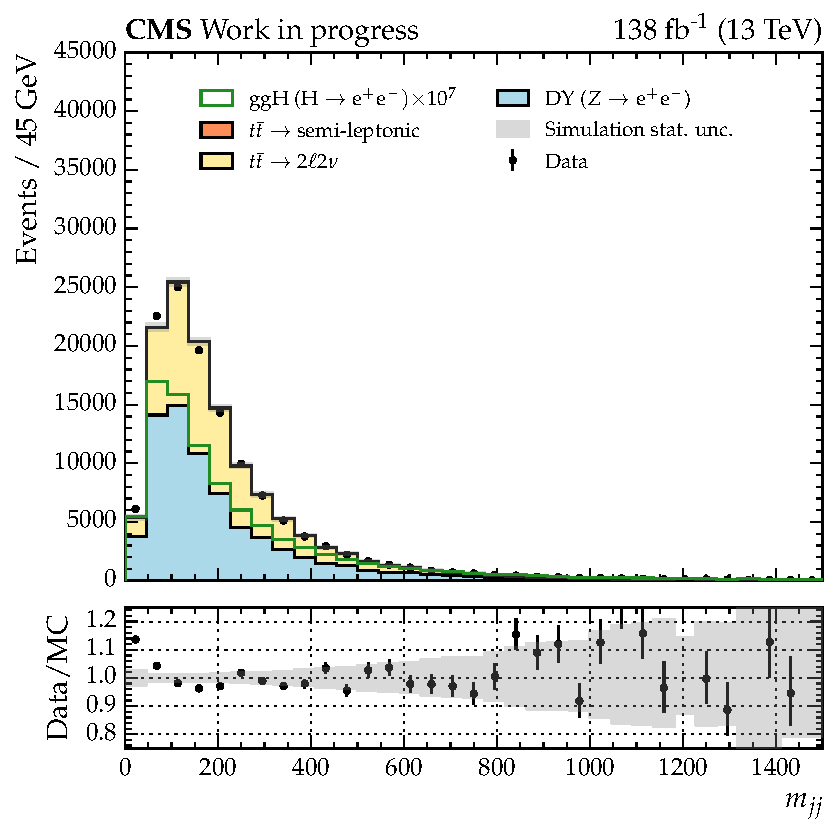
\includegraphics[width =0.33\linewidth]{Figures/Hee/ggH/dataMC/all_inputs/ggH_BDT_pt_reweighted_dijetMass.pdf}\hfill%
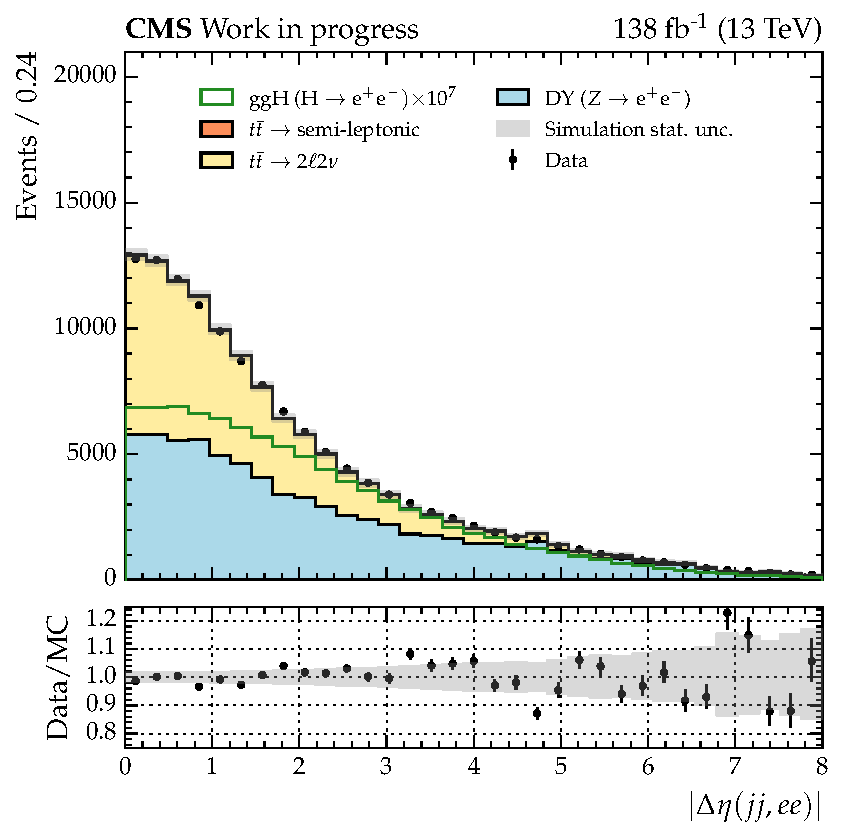
\includegraphics[width =0.33\linewidth]{Figures/Hee/ggH/dataMC/all_inputs/ggH_BDT_pt_reweighted_dijetDieleAbsDEta.pdf}\hfill%
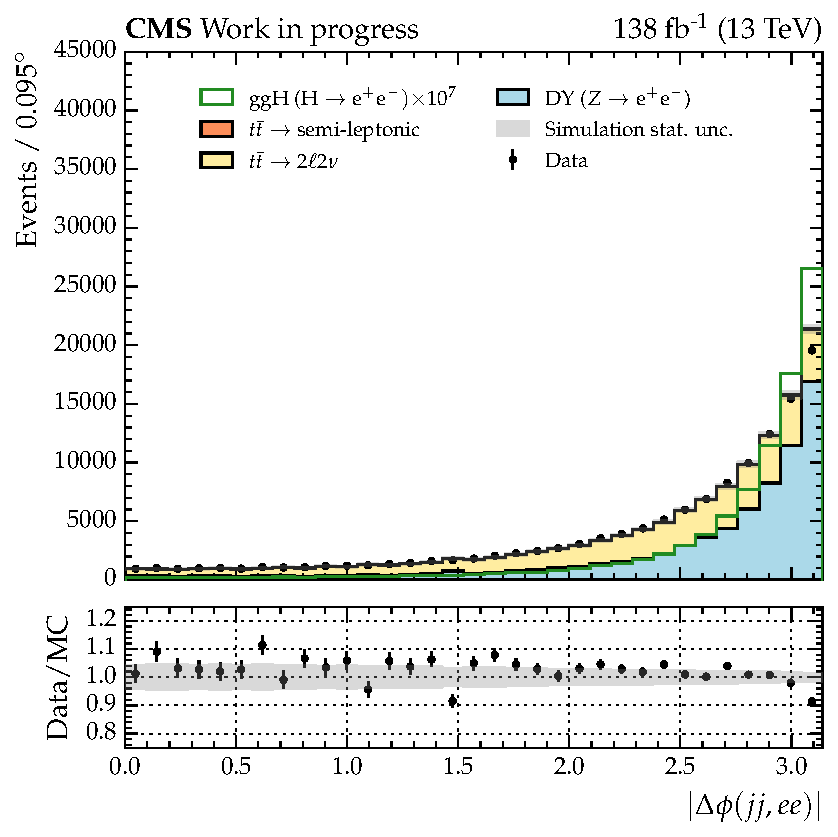
\includegraphics[width =0.33\linewidth]{Figures/Hee/ggH/dataMC/all_inputs/ggH_BDT_pt_reweighted_dijetDieleAbsDPhiTrunc.pdf}\hfill%
 
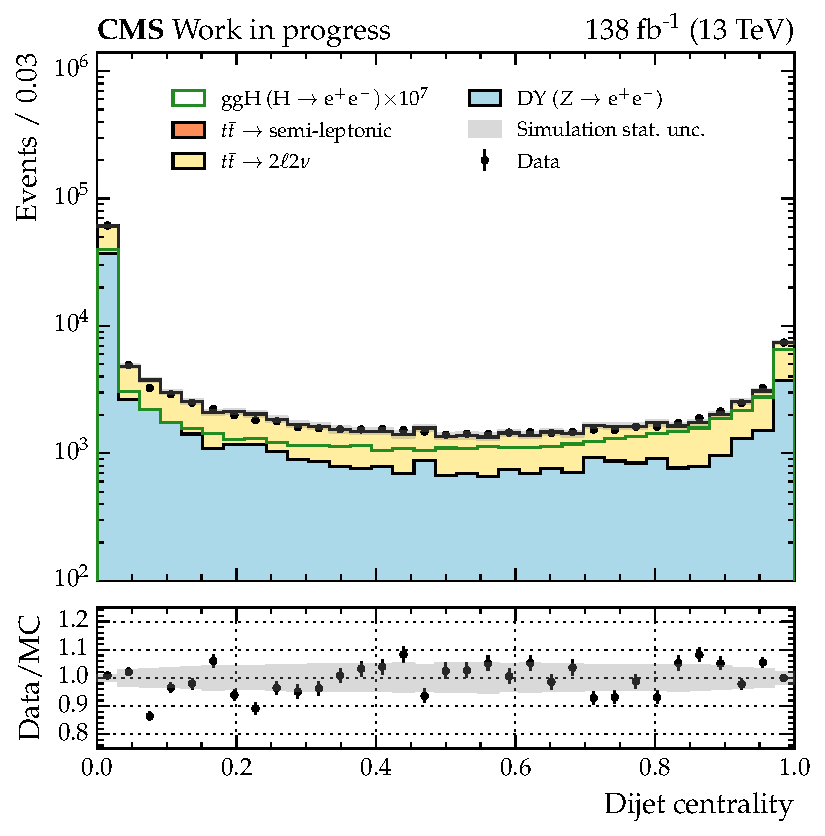
\includegraphics[width =0.33\linewidth]{Figures/Hee/ggH/dataMC/all_inputs/ggH_BDT_pt_reweighted_dijetCentrality.pdf}\hfill%
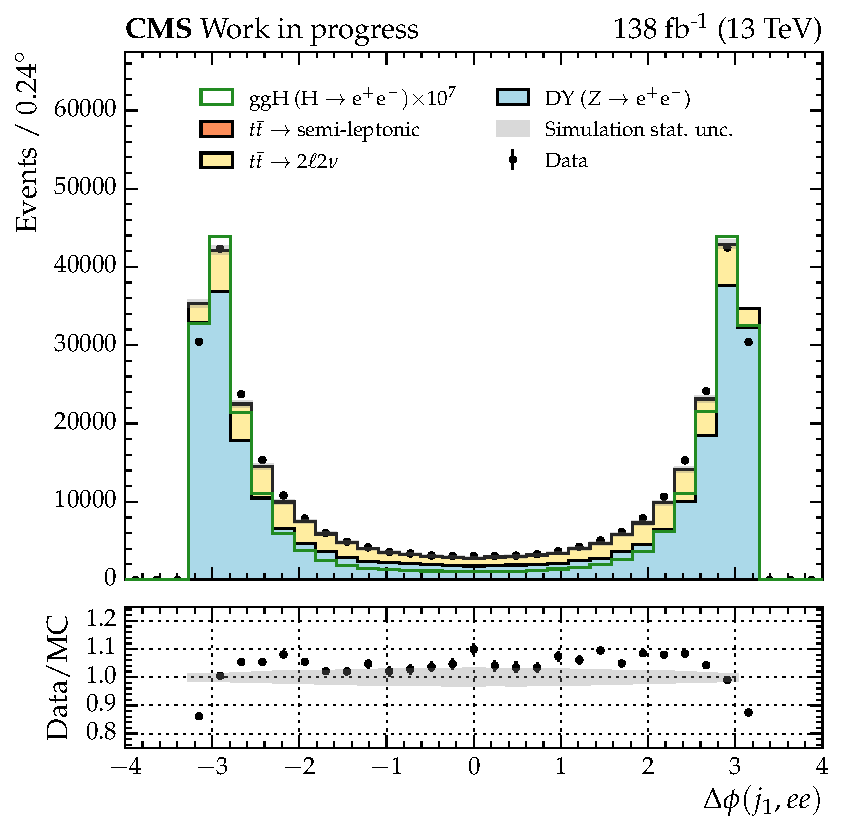
\includegraphics[width =0.33\linewidth]{Figures/Hee/ggH/dataMC/all_inputs/ggH_BDT_pt_reweighted_leadJetDieleDPhi.pdf}\hfill%
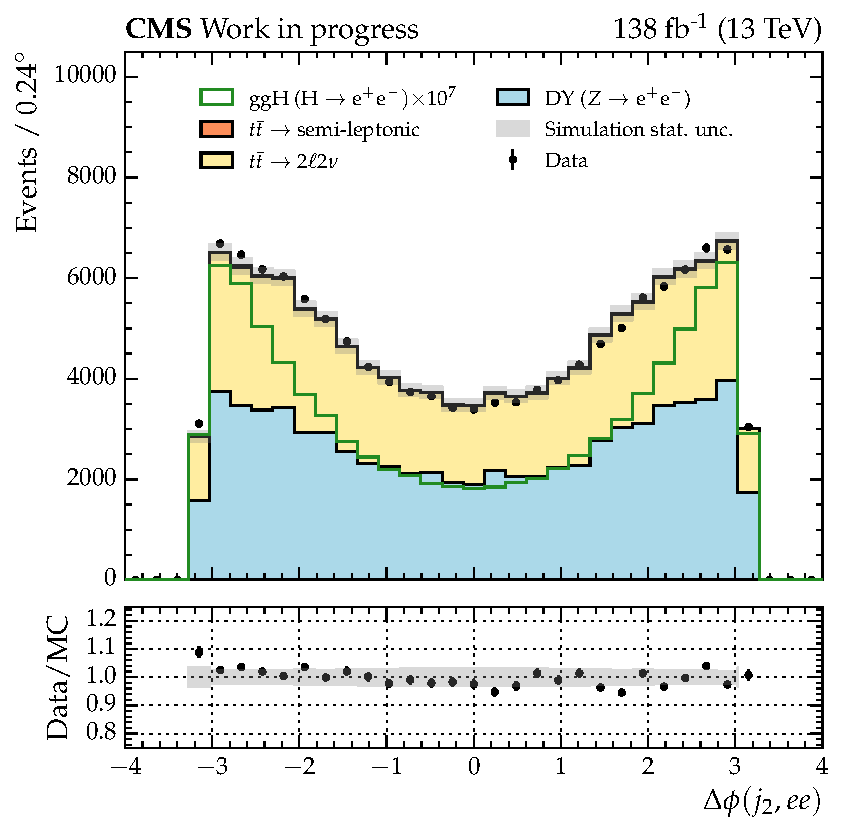
\includegraphics[width =0.33\linewidth]{Figures/Hee/ggH/dataMC/all_inputs/ggH_BDT_pt_reweighted_subleadJetDieleDPhi.pdf}\hfill%
 
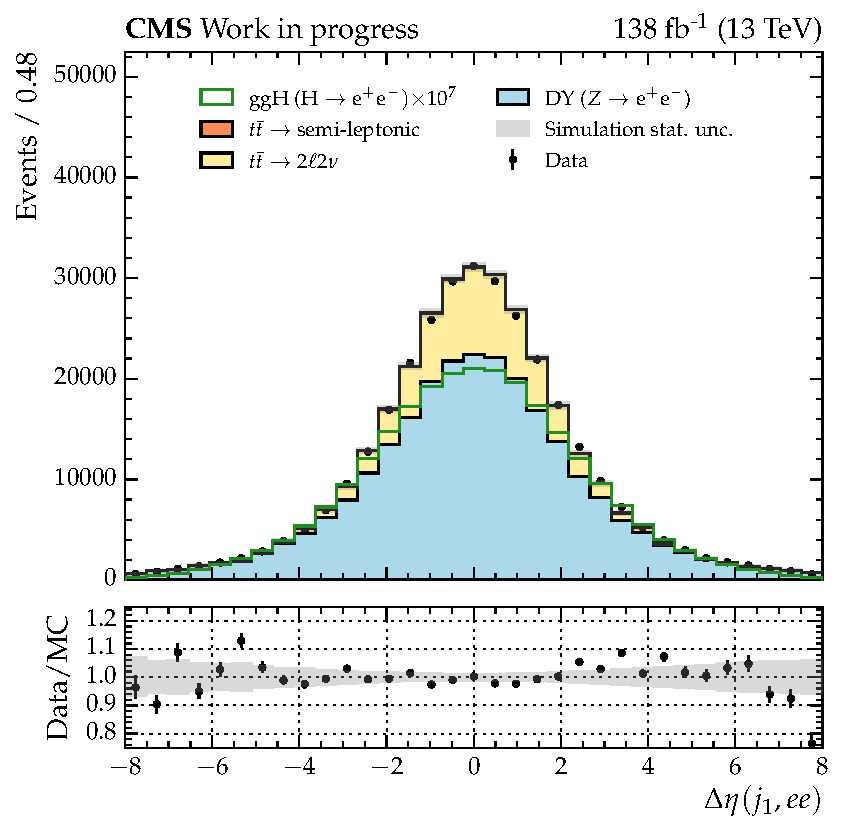
\includegraphics[width =0.33\linewidth]{Figures/Hee/ggH/dataMC/all_inputs/ggH_BDT_pt_reweighted_leadJetDieleDEta.pdf}\hfill%
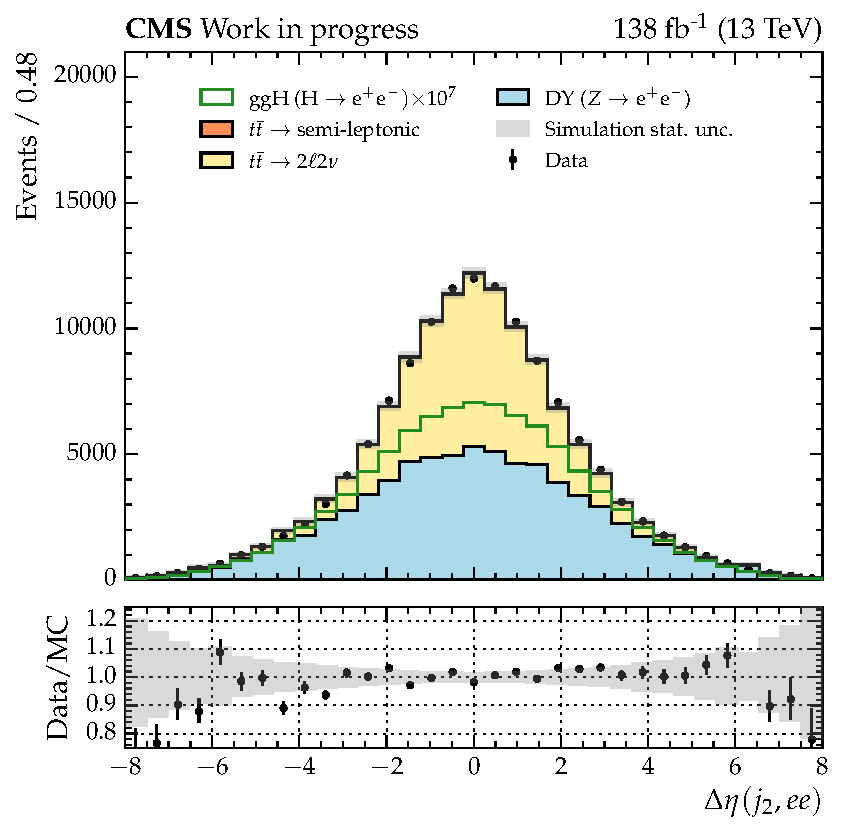
\includegraphics[width =0.33\linewidth]{Figures/Hee/ggH/dataMC/all_inputs/ggH_BDT_pt_reweighted_subleadJetDieleDEta.pdf}\hfill%
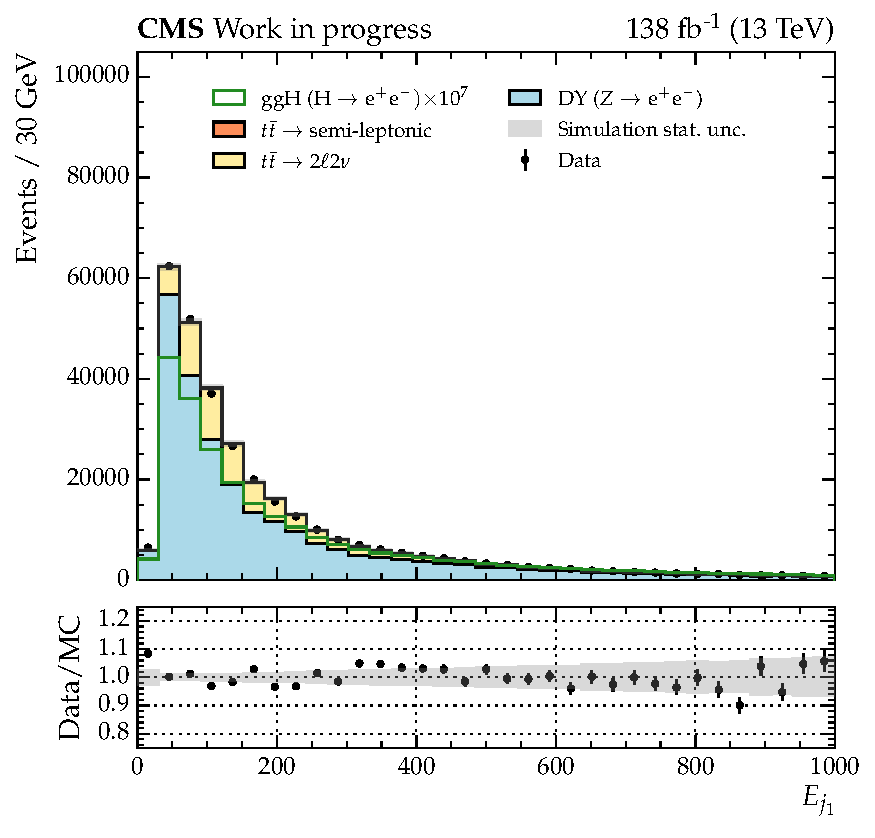
\includegraphics[width =0.33\linewidth]{Figures/Hee/ggH/dataMC/all_inputs/ggH_BDT_pt_reweighted_leadJetEn.pdf}\hfill% 
 
\caption{Distributions for the input variables to the gluon-fusion BDT. The ggH signal is shown in green, with the overall normalisation scaled such that it is visible. The simulated background processes (bold face) are stacked for comparison with data (black points). Reasonable agreement is observed between data and simulation, with respect to the statistical uncertainty (grey band).}
\label{fig:ggH_inputs_second}
\end{figure}
 
\begin{figure}[htbp!]
\centering
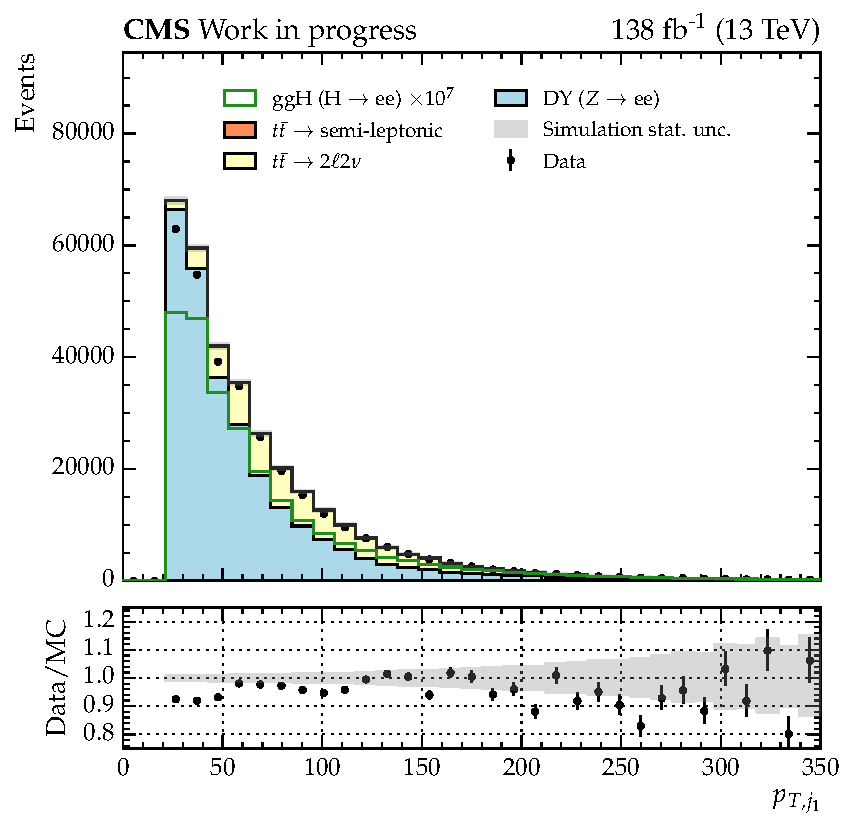
\includegraphics[width =0.33\linewidth]{Figures/Hee/ggH/dataMC/all_inputs/ggH_BDT_pt_reweighted_leadJetPt.pdf}\hfill%
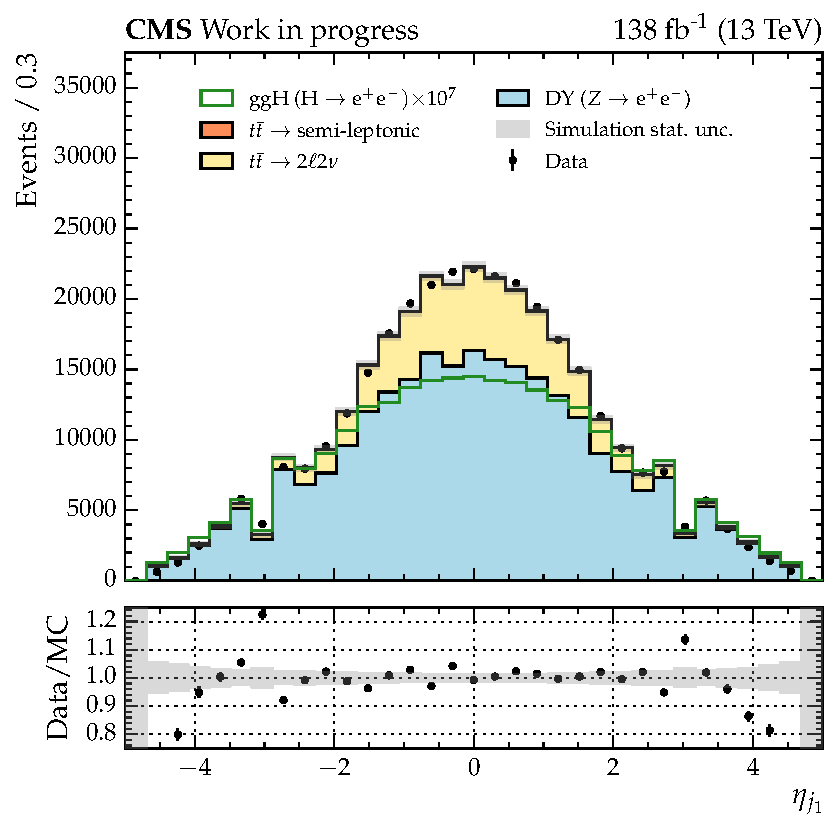
\includegraphics[width =0.33\linewidth]{Figures/Hee/ggH/dataMC/all_inputs/ggH_BDT_pt_reweighted_leadJetEta.pdf}\hfill%
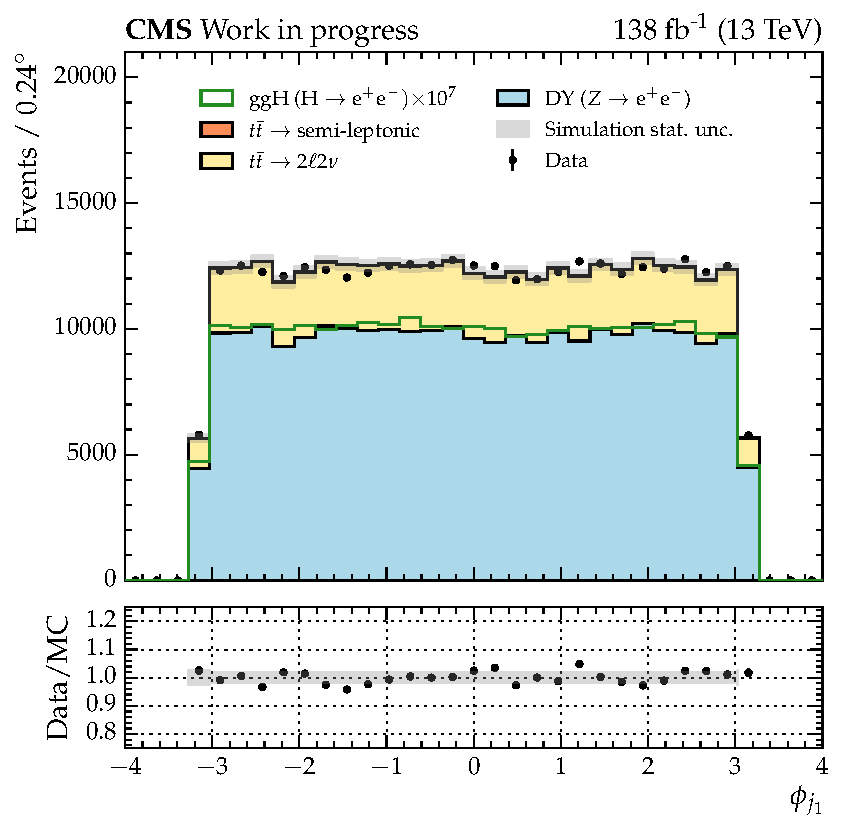
\includegraphics[width =0.33\linewidth]{Figures/Hee/ggH/dataMC/all_inputs/ggH_BDT_pt_reweighted_leadJetPhi.pdf}\hfill%
 
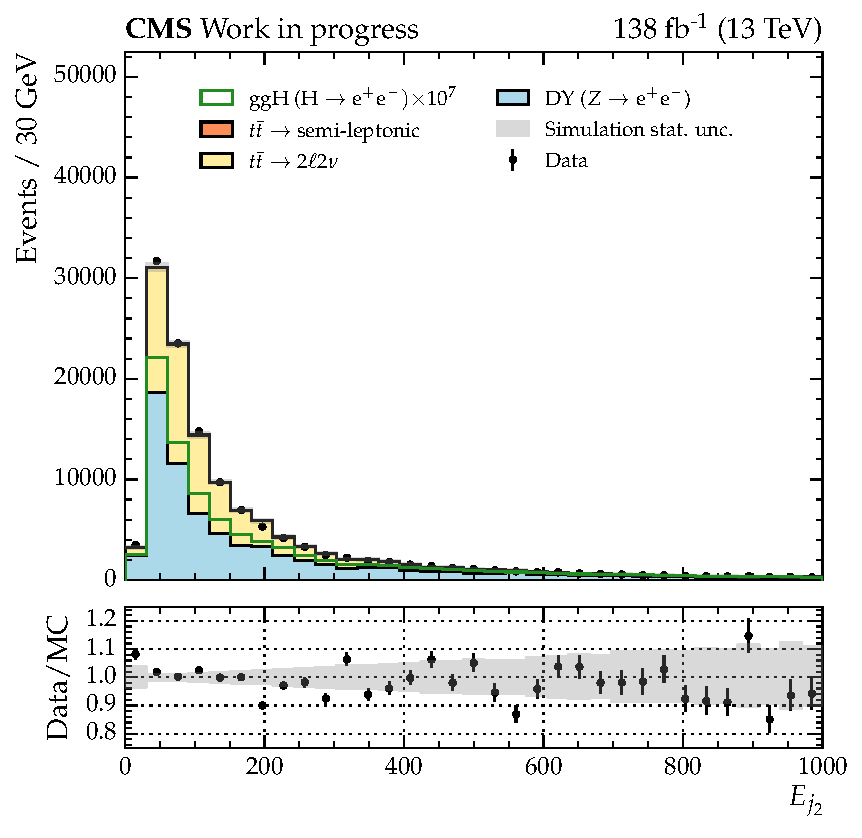
\includegraphics[width =0.33\linewidth]{Figures/Hee/ggH/dataMC/all_inputs/ggH_BDT_pt_reweighted_subleadJetEn.pdf}\hfill%
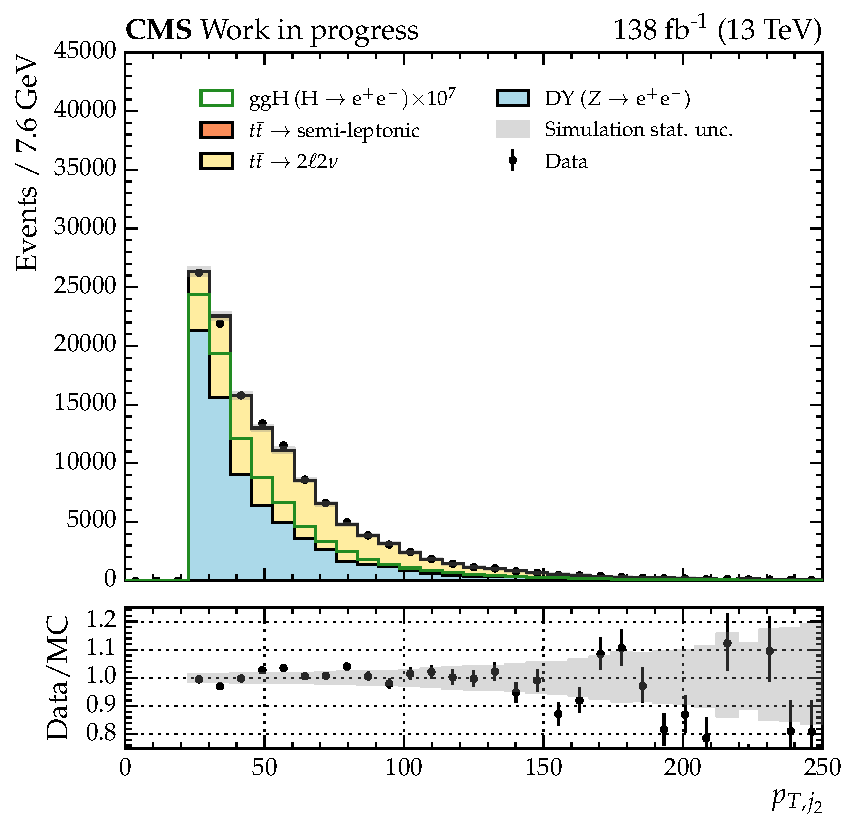
\includegraphics[width =0.33\linewidth]{Figures/Hee/ggH/dataMC/all_inputs/ggH_BDT_pt_reweighted_subleadJetPt.pdf}\hfill%
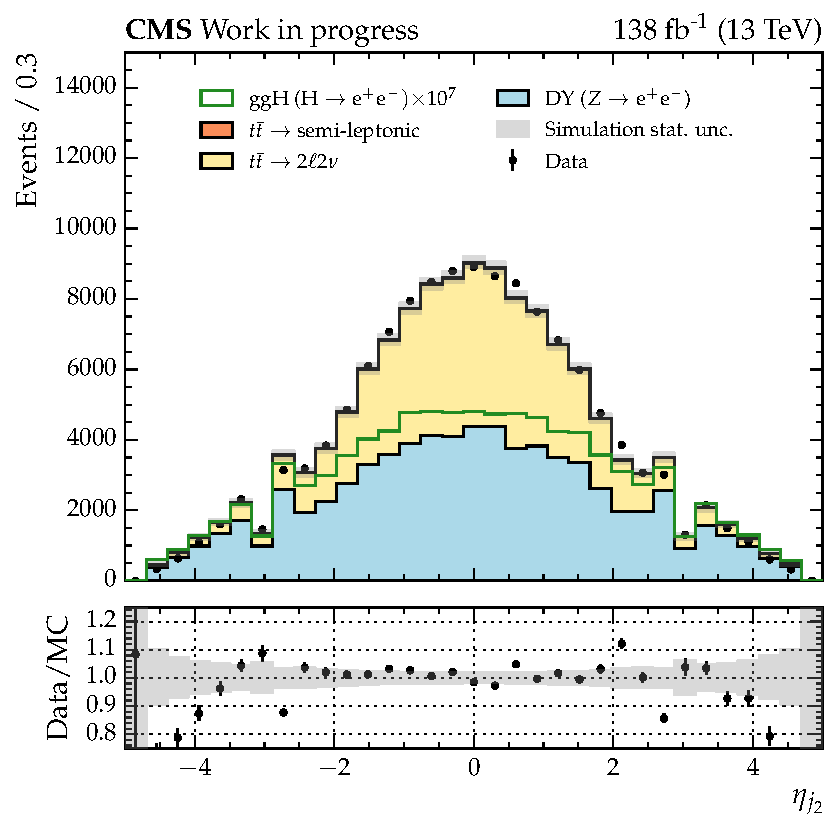
\includegraphics[width =0.33\linewidth]{Figures/Hee/ggH/dataMC/all_inputs/ggH_BDT_pt_reweighted_subleadJetEta.pdf}\hfill%
 
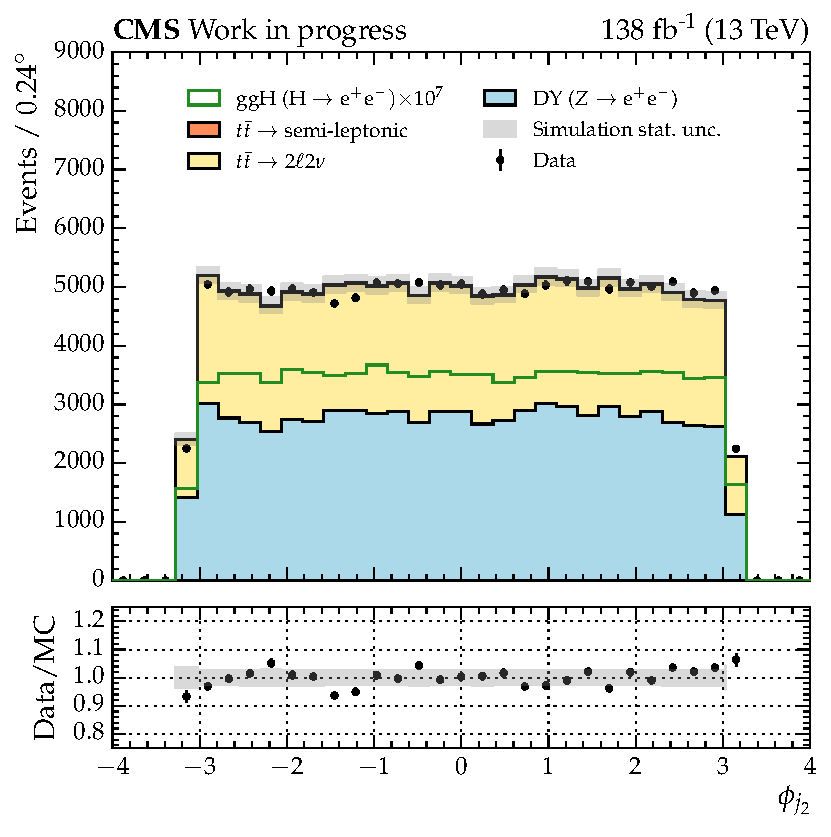
\includegraphics[width =0.33\linewidth]{Figures/Hee/ggH/dataMC/all_inputs/ggH_BDT_pt_reweighted_subleadJetPhi.pdf}\hfill%
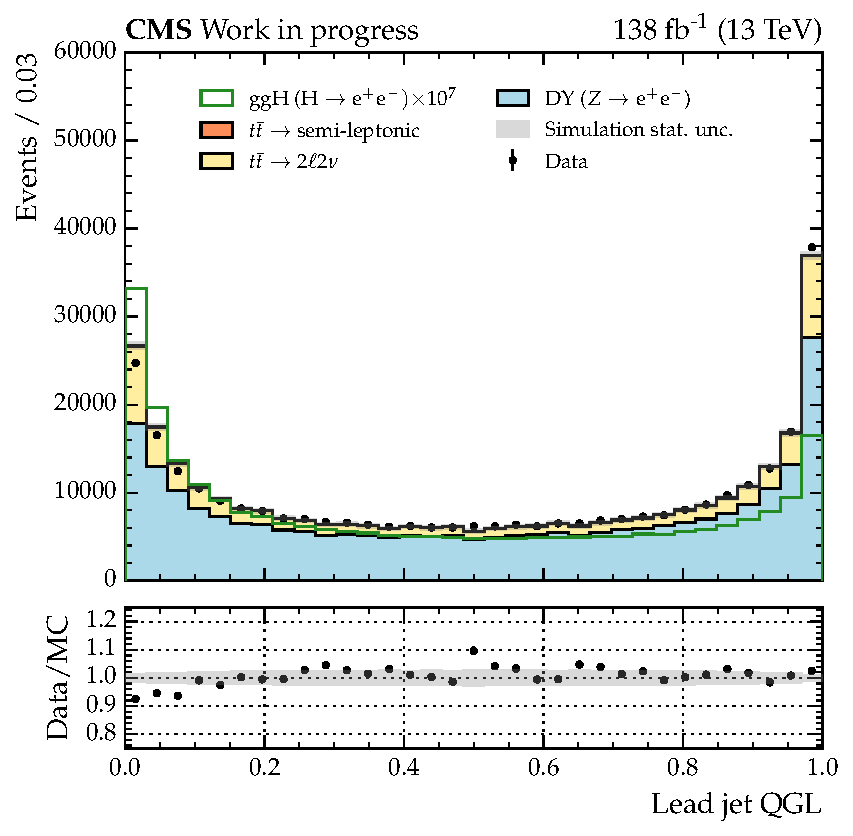
\includegraphics[width =0.33\linewidth]{Figures/Hee/ggH/dataMC/all_inputs/ggH_BDT_pt_reweighted_leadJetQGL.pdf}\hfill%
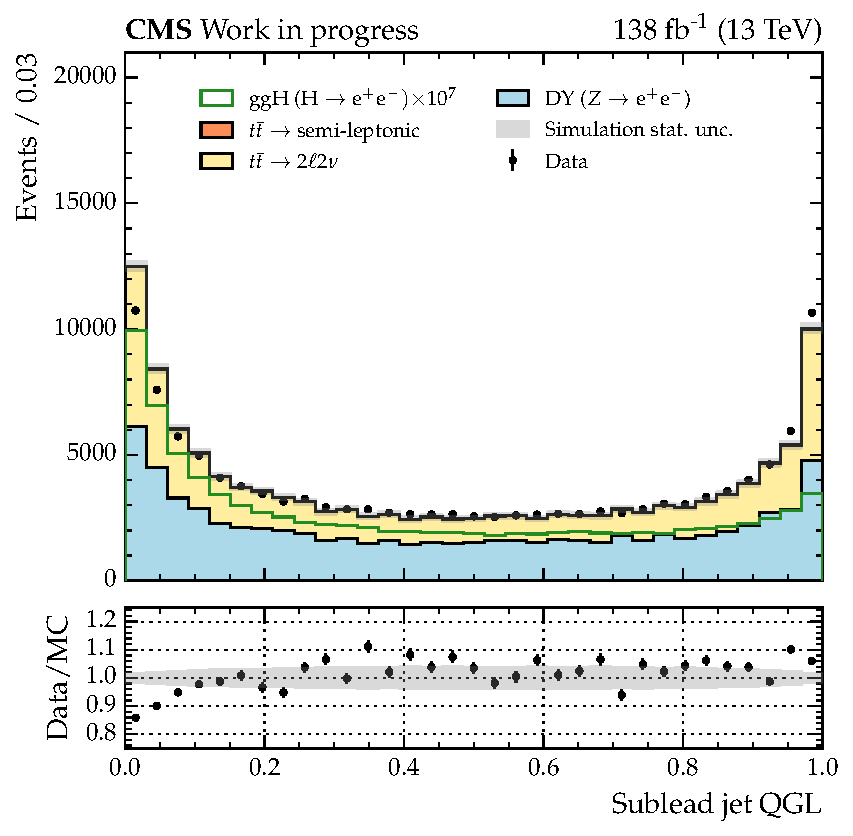
\includegraphics[width =0.33\linewidth]{Figures/Hee/ggH/dataMC/all_inputs/ggH_BDT_pt_reweighted_subleadJetQGL.pdf}\hfill%
 
\caption{Distributions for the input variables to the gluon-fusion BDT. The ggH signal is shown in green, with the overall normalisation scaled such that it is visible. The simulated background processes (bold face) are stacked for comparison with data (black points). Reasonable agreement is observed between data and simulation, with respect to the statistical uncertainty (grey band).}
\label{fig:ggH_inputs_last}
\end{figure}



%%%VBF%%%

\begin{figure}[htbp!]
\centering
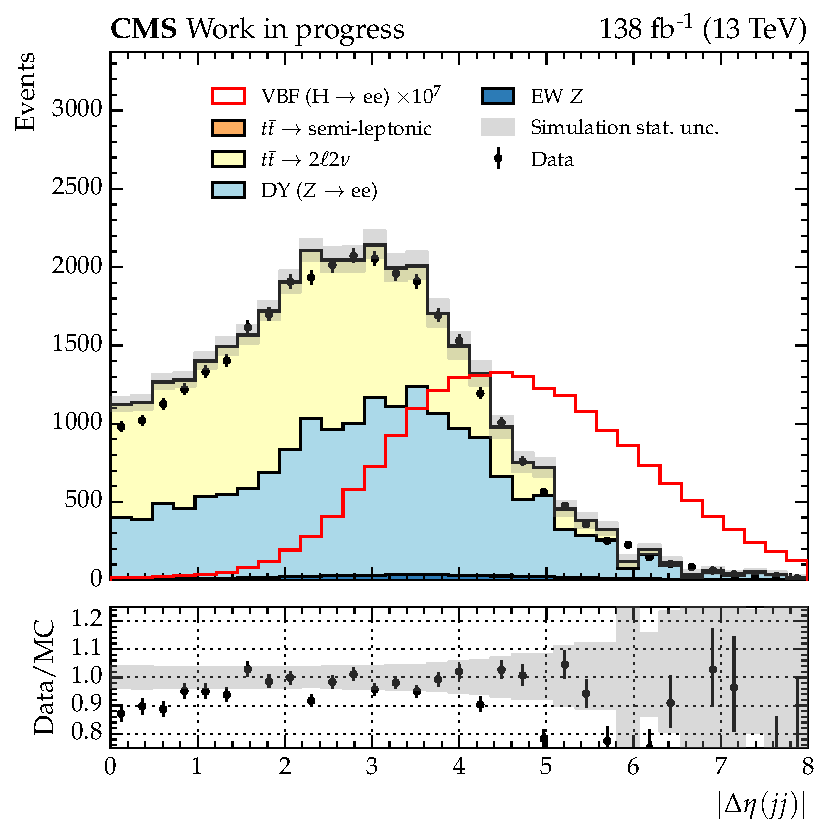
\includegraphics[width =0.33\linewidth]{Figures/Hee/VBF/dataMC/all_inputs/VBF_BDT_dijetAbsDEta.pdf}\hfill%
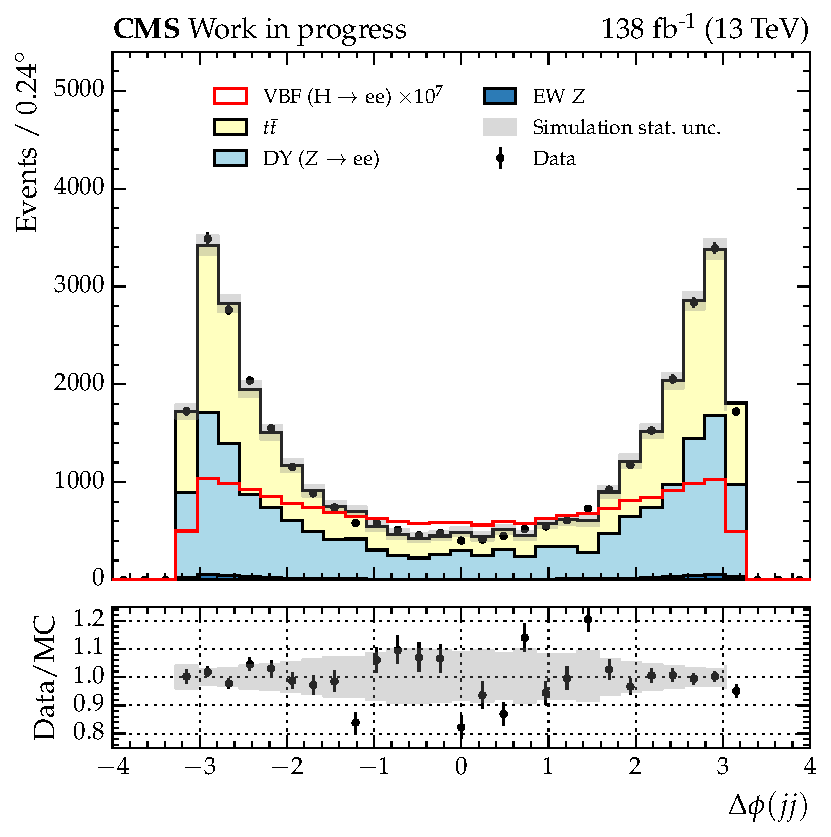
\includegraphics[width =0.33\linewidth]{Figures/Hee/VBF/dataMC/all_inputs/VBF_BDT_dijetDPhi.pdf}\hfill%
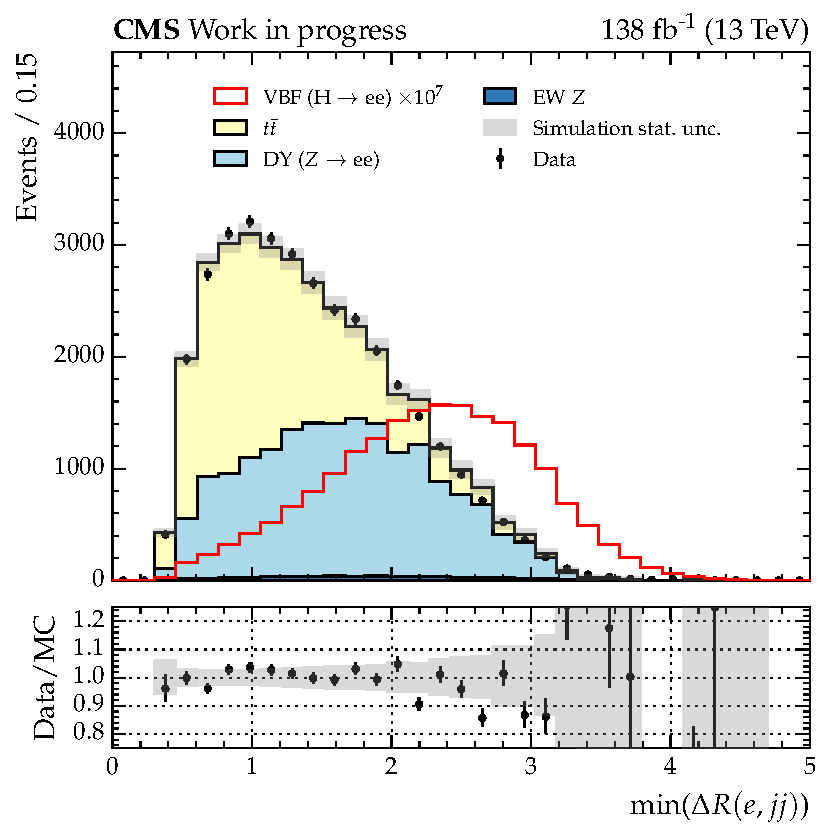
\includegraphics[width =0.33\linewidth]{Figures/Hee/VBF/dataMC/all_inputs/VBF_BDT_dijetMinDRJetEle.pdf}\hfill%
 
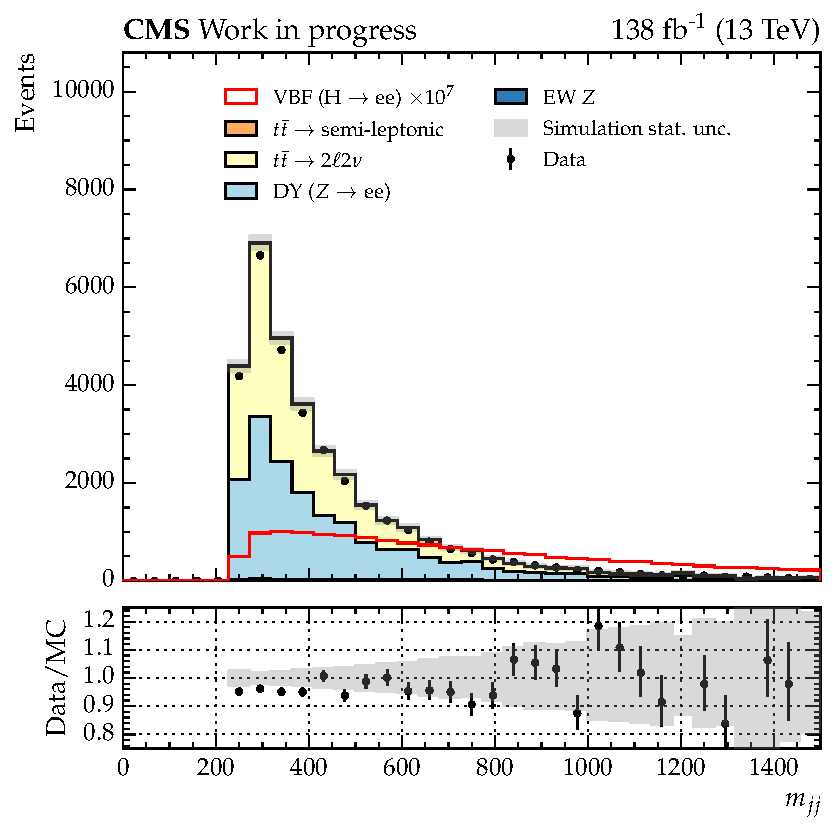
\includegraphics[width =0.33\linewidth]{Figures/Hee/VBF/dataMC/all_inputs/VBF_BDT_dijetMass.pdf}\hfill%
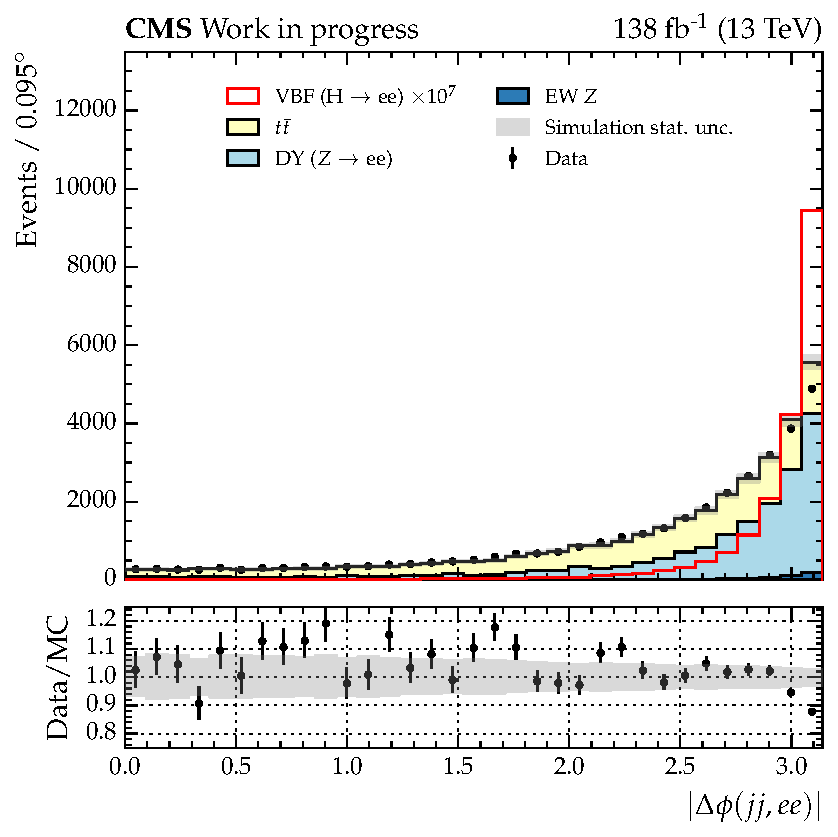
\includegraphics[width =0.33\linewidth]{Figures/Hee/VBF/dataMC/all_inputs/VBF_BDT_dijetDieleAbsDPhiTrunc.pdf}\hfill%
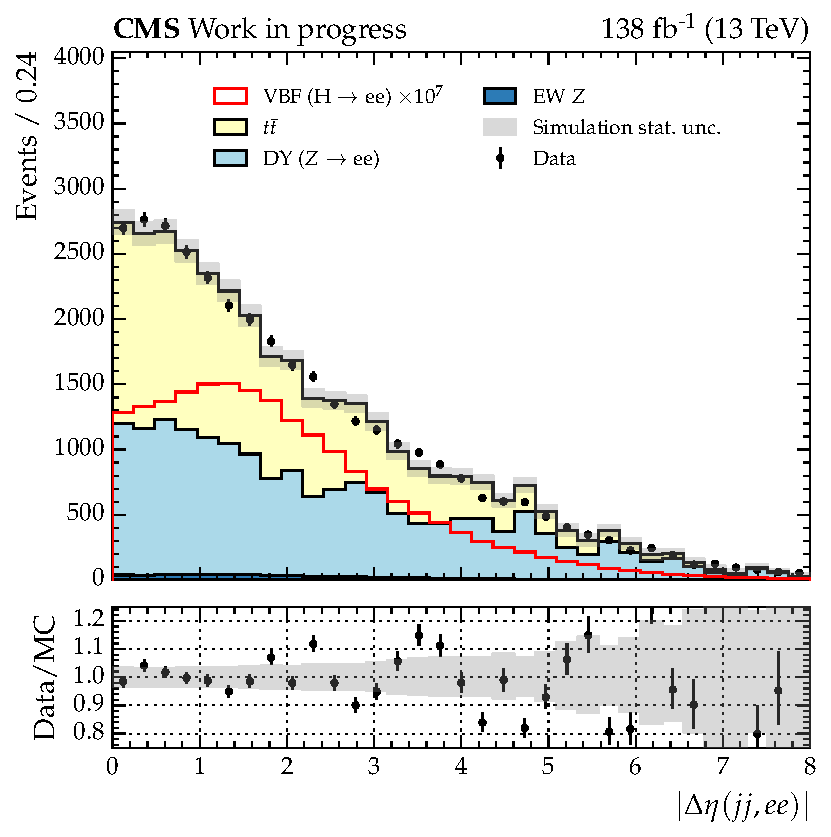
\includegraphics[width =0.33\linewidth]{Figures/Hee/VBF/dataMC/all_inputs/VBF_BDT_dijetDieleAbsDEta.pdf}\hfill%
\caption{Distributions for the input variables to the VBF BDT. The VBF signal is shown in red, with the overall normalisation scaled such that it is visible. The simulated background processes (bold face) are stacked for comparison with data (black points). Good agreement is observed between data and simulation, with respect to the statistical uncertainty (grey band).} 
\label{fig:VBF_inputs_first}
\end{figure}
 
\begin{figure}[htbp!]
\centering
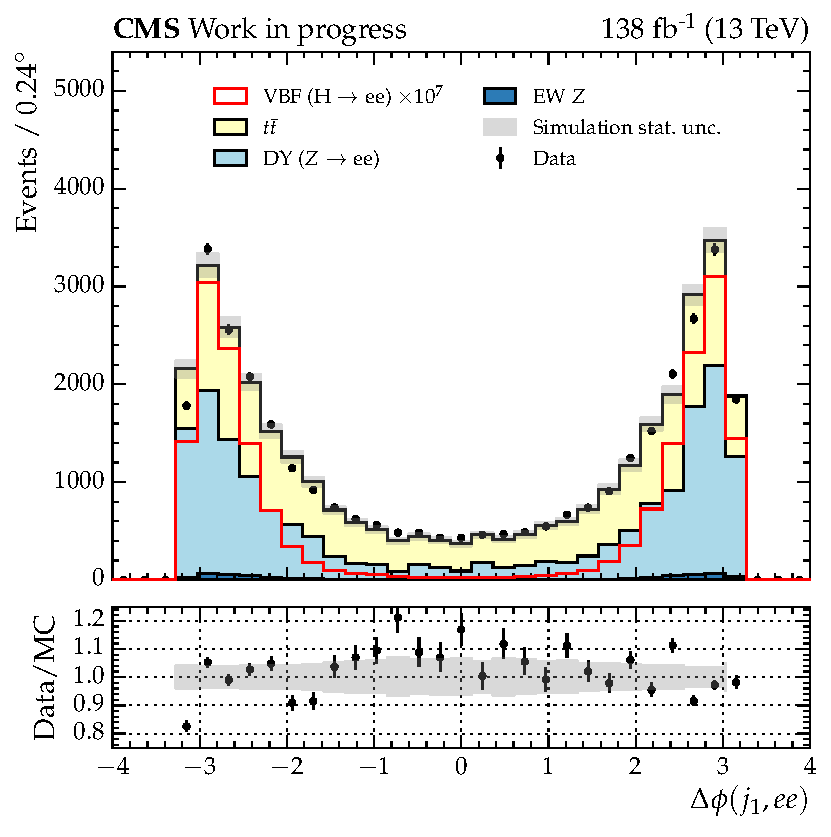
\includegraphics[width =0.33\linewidth]{Figures/Hee/VBF/dataMC/all_inputs/VBF_BDT_leadJetDieleDPhi.pdf}\hfill%
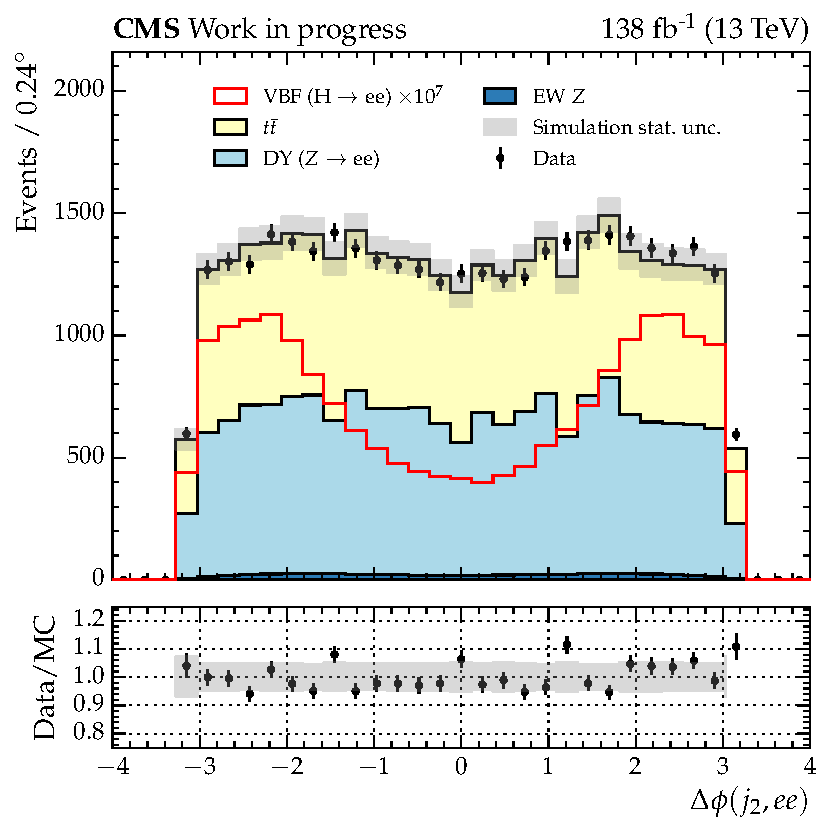
\includegraphics[width =0.33\linewidth]{Figures/Hee/VBF/dataMC/all_inputs/VBF_BDT_subleadJetDieleDPhi.pdf}\hfill%
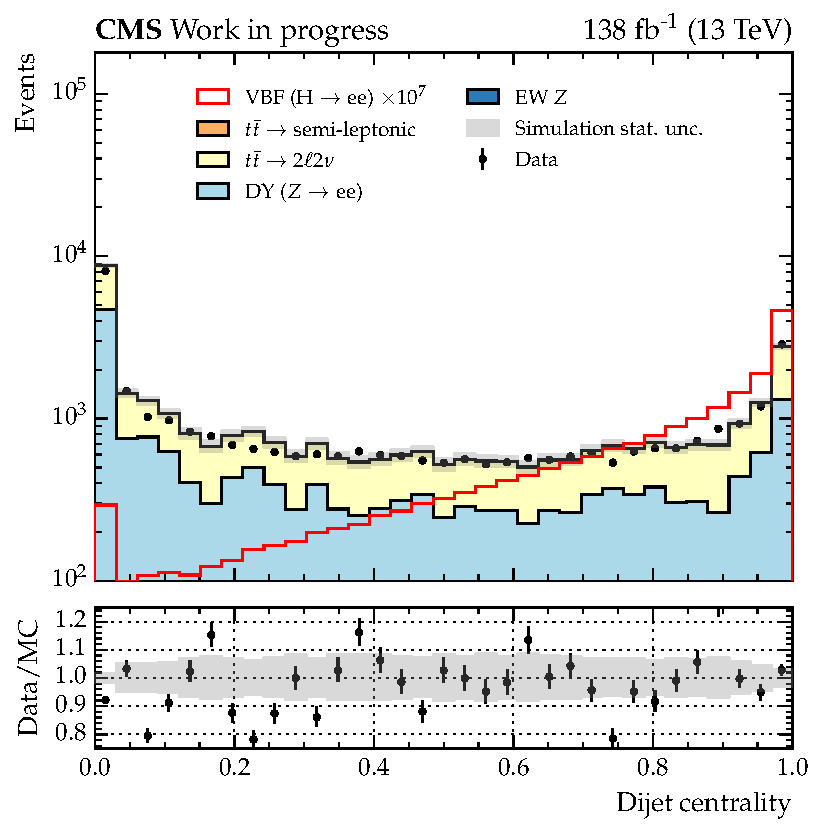
\includegraphics[width =0.33\linewidth]{Figures/Hee/VBF/dataMC/all_inputs/VBF_BDT_dijetCentrality.pdf}\hfill%
 
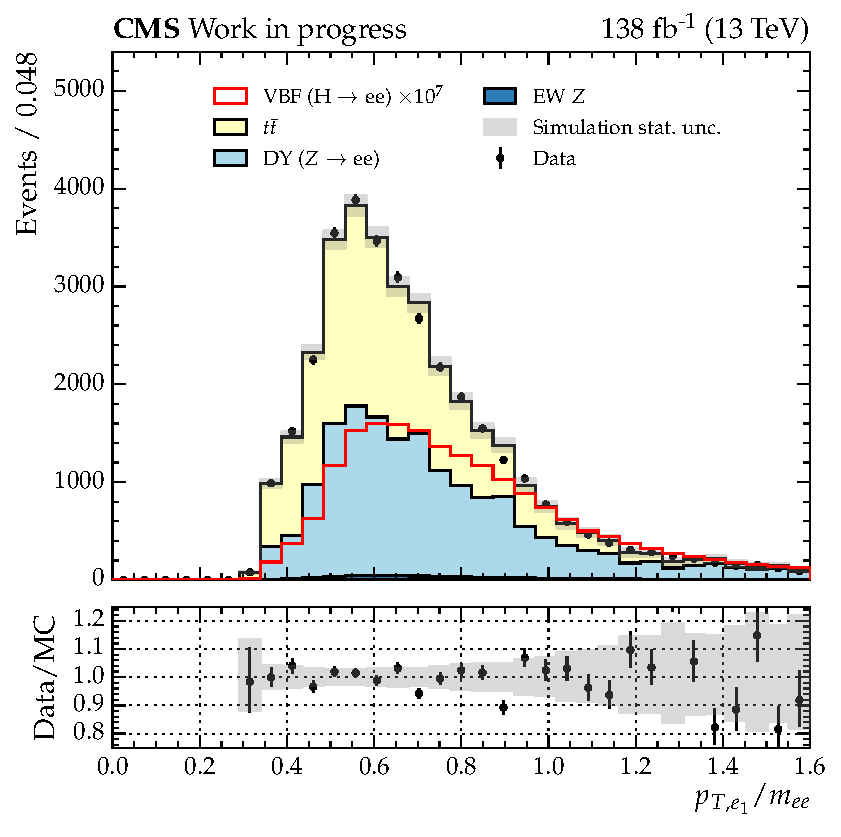
\includegraphics[width =0.33\linewidth]{Figures/Hee/VBF/dataMC/all_inputs/VBF_BDT_leadElectronPtOvM.pdf}\hfill%
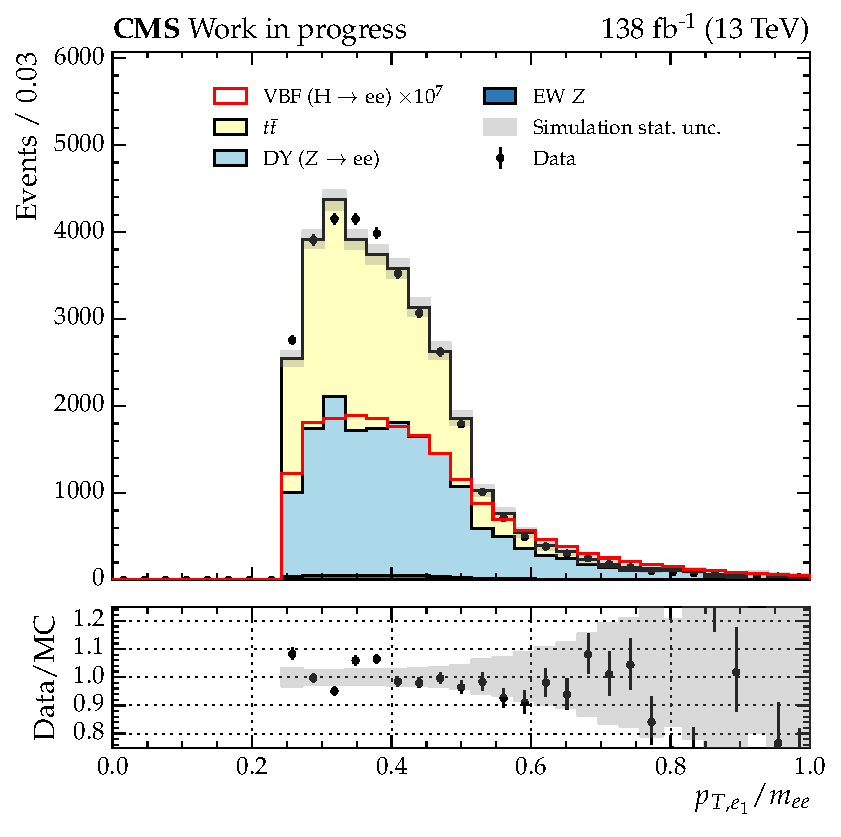
\includegraphics[width =0.33\linewidth]{Figures/Hee/VBF/dataMC/all_inputs/VBF_BDT_subleadElectronPtOvM.pdf}\hfill%
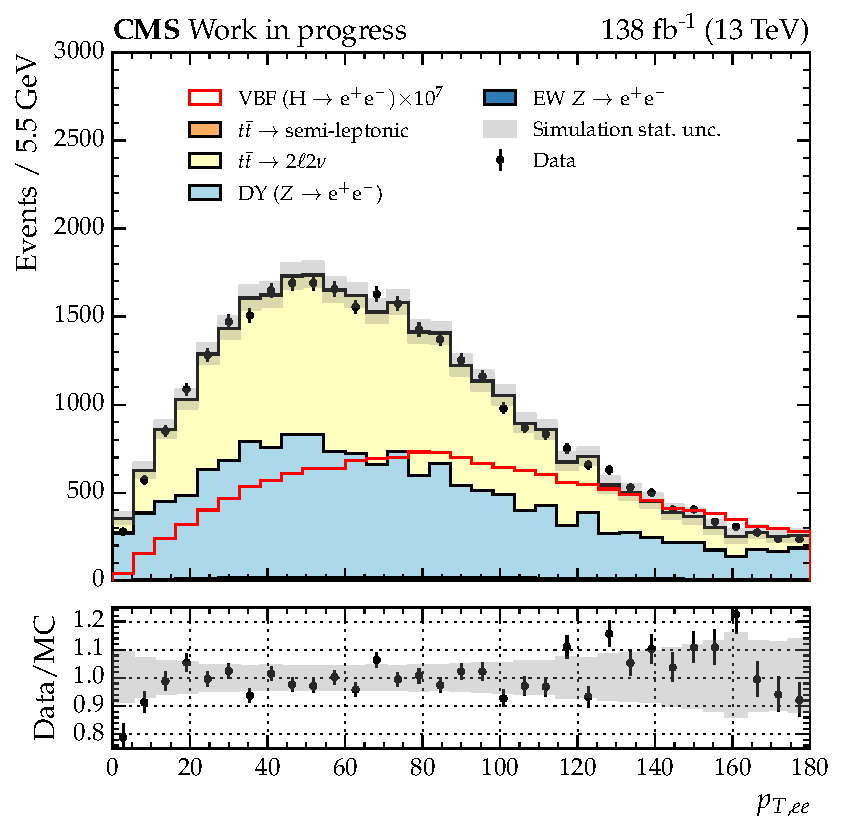
\includegraphics[width =0.33\linewidth]{Figures/Hee/VBF/dataMC/all_inputs/VBF_BDT_dielectronPt.pdf}\hfill%
\caption{Distributions for the input variables to the VBF BDT. The VBF signal is shown in red, with the overall normalisation scaled such that it is visible. The simulated background processes (bold face) are stacked for comparison with data (black points). Good agreement is observed between data and simulation, with respect to the statistical uncertainty (grey band).} 
\end{figure}
 
 
\begin{figure}[htbp!]
\centering
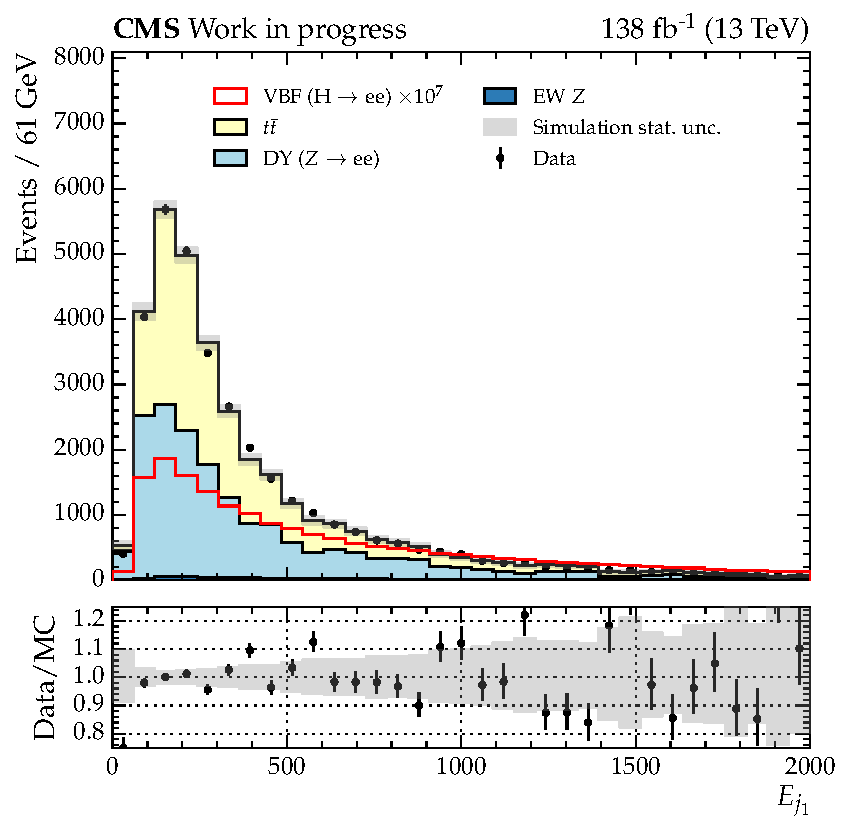
\includegraphics[width =0.33\linewidth]{Figures/Hee/VBF/dataMC/all_inputs/VBF_BDT_leadJetEn.pdf}\hfill%
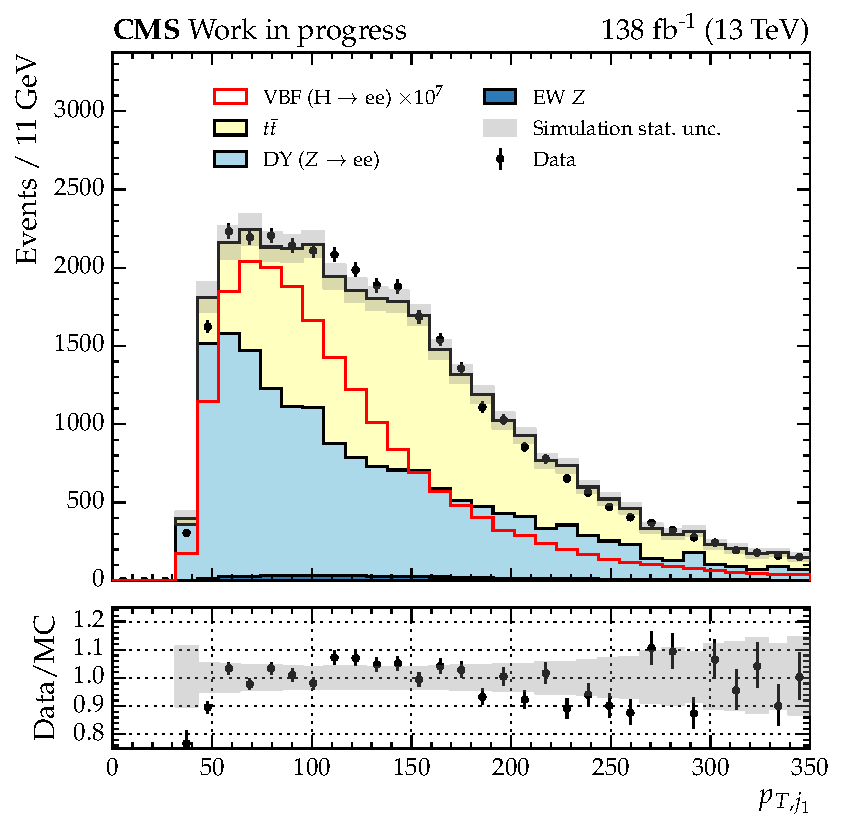
\includegraphics[width =0.33\linewidth]{Figures/Hee/VBF/dataMC/all_inputs/VBF_BDT_leadJetPt.pdf}\hfill%
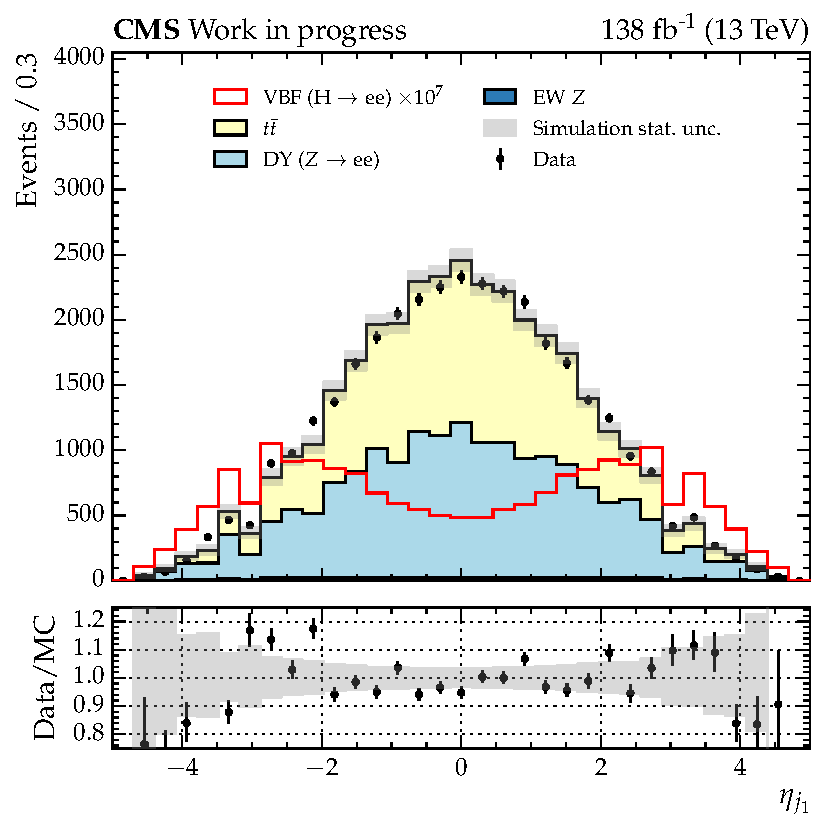
\includegraphics[width =0.33\linewidth]{Figures/Hee/VBF/dataMC/all_inputs/VBF_BDT_leadJetEta.pdf}\hfill%
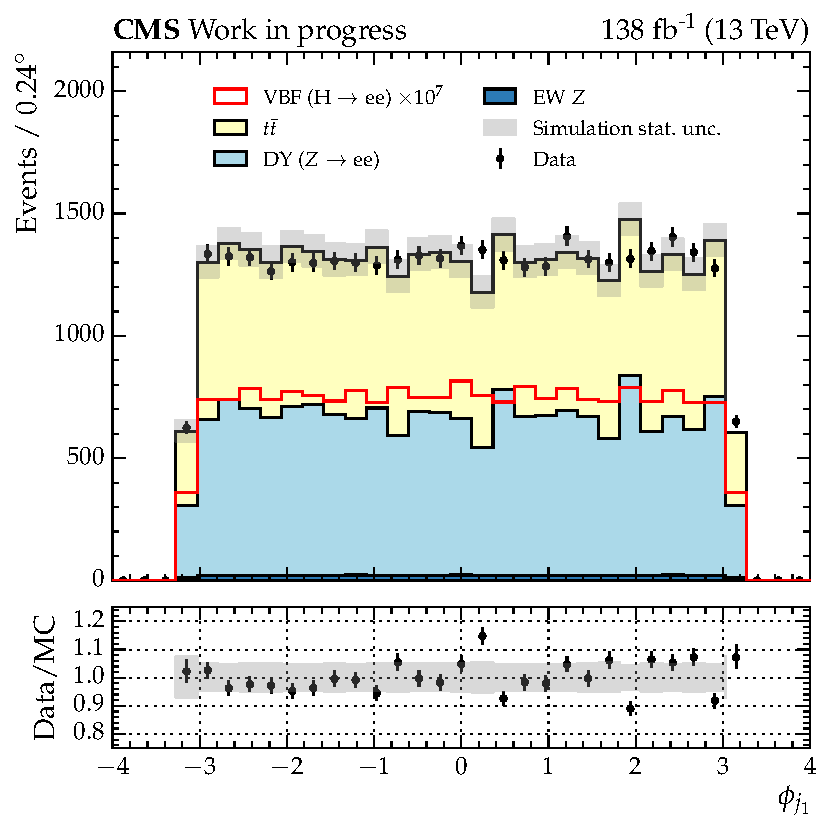
\includegraphics[width =0.33\linewidth]{Figures/Hee/VBF/dataMC/all_inputs/VBF_BDT_leadJetPhi.pdf}
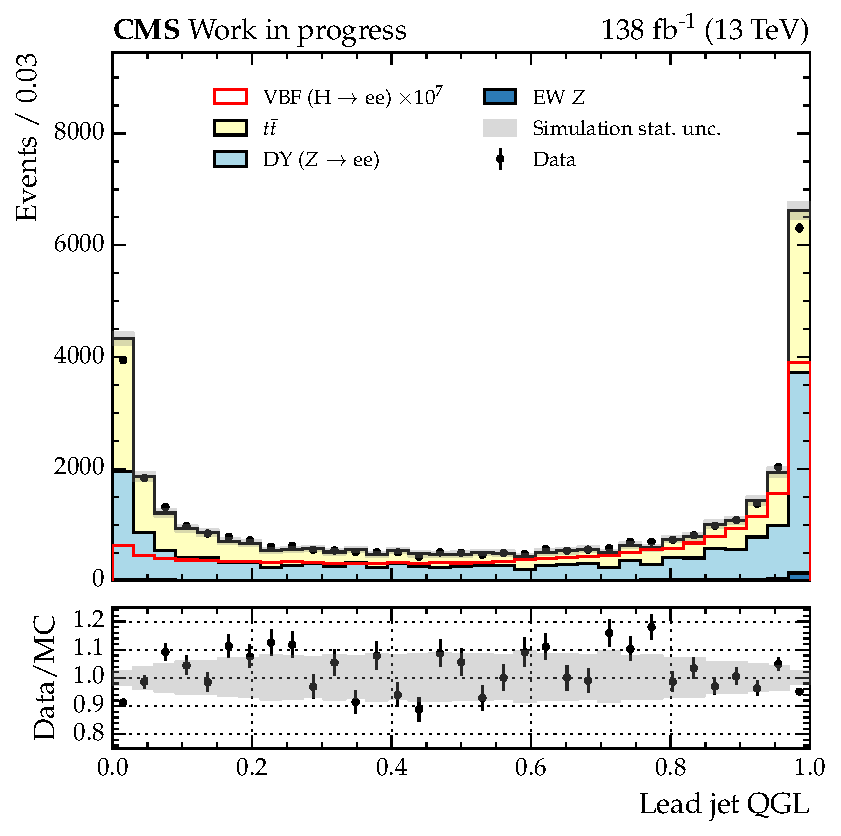
\includegraphics[width =0.33\linewidth]{Figures/Hee/VBF/dataMC/all_inputs/VBF_BDT_leadJetQGL.pdf}\hfill%
\caption{Distributions for the input variables to the VBF BDT. The VBF signal is shown in red, with the overall normalisation scaled such that it is visible. The simulated background processes (bold face) are stacked for comparison with data (black points). Good agreement is observed between data and simulation, with respect to the statistical uncertainty (grey band).} 
\end{figure}
 
 
\begin{figure}[htbp!]
\centering
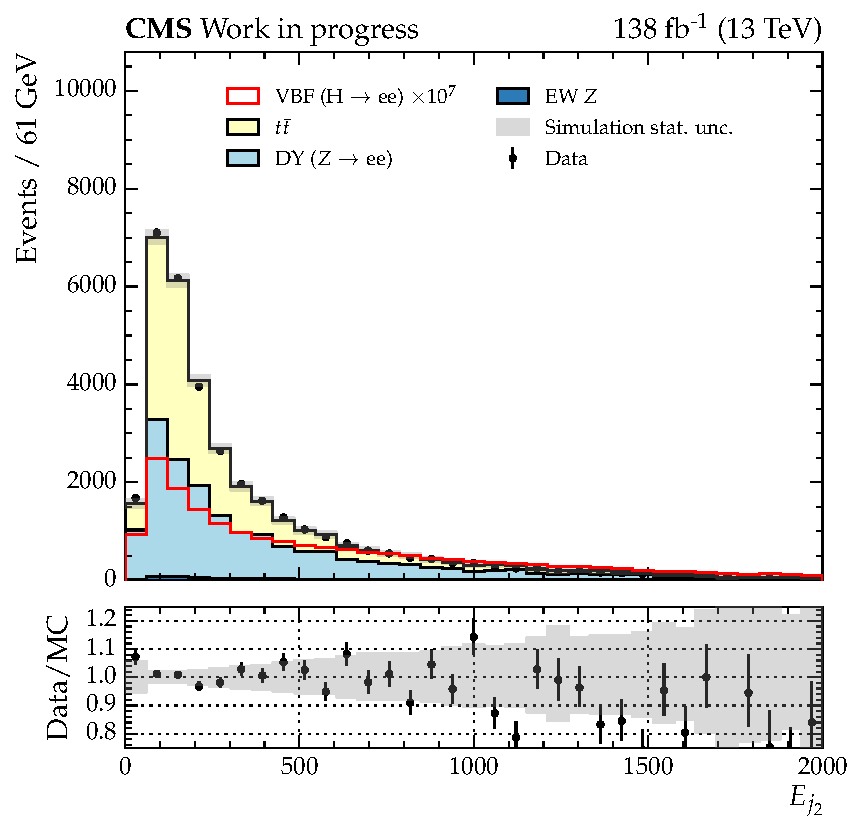
\includegraphics[width =0.33\linewidth]{Figures/Hee/VBF/dataMC/all_inputs/VBF_BDT_subleadJetEn.pdf}\hfill%
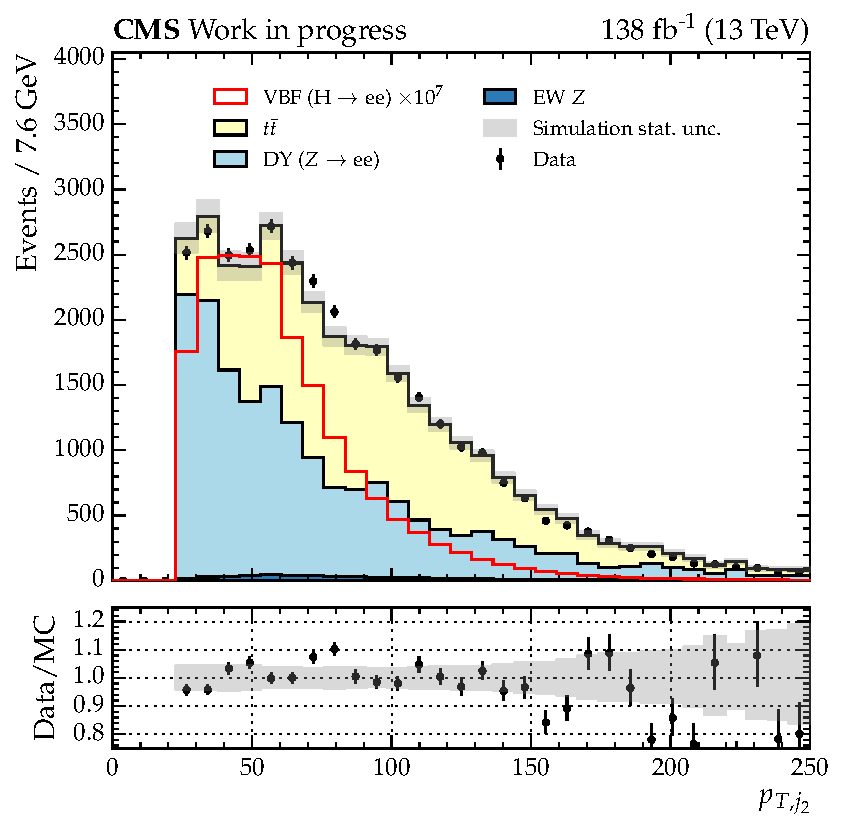
\includegraphics[width =0.33\linewidth]{Figures/Hee/VBF/dataMC/all_inputs/VBF_BDT_subleadJetPt.pdf}\hfill%
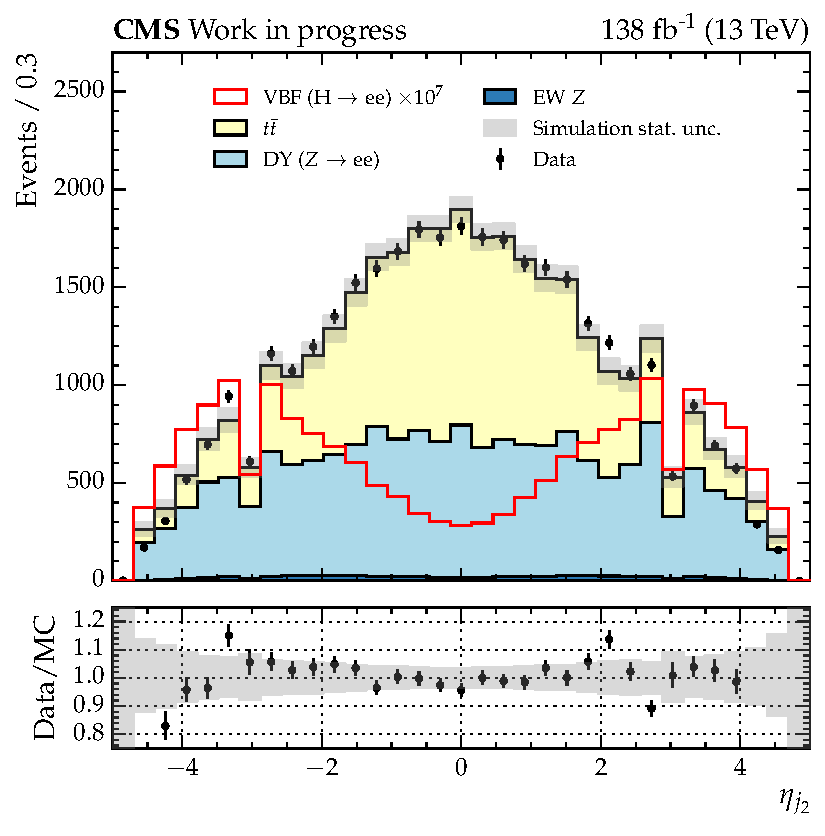
\includegraphics[width =0.33\linewidth]{Figures/Hee/VBF/dataMC/all_inputs/VBF_BDT_subleadJetEta.pdf}\hfill%
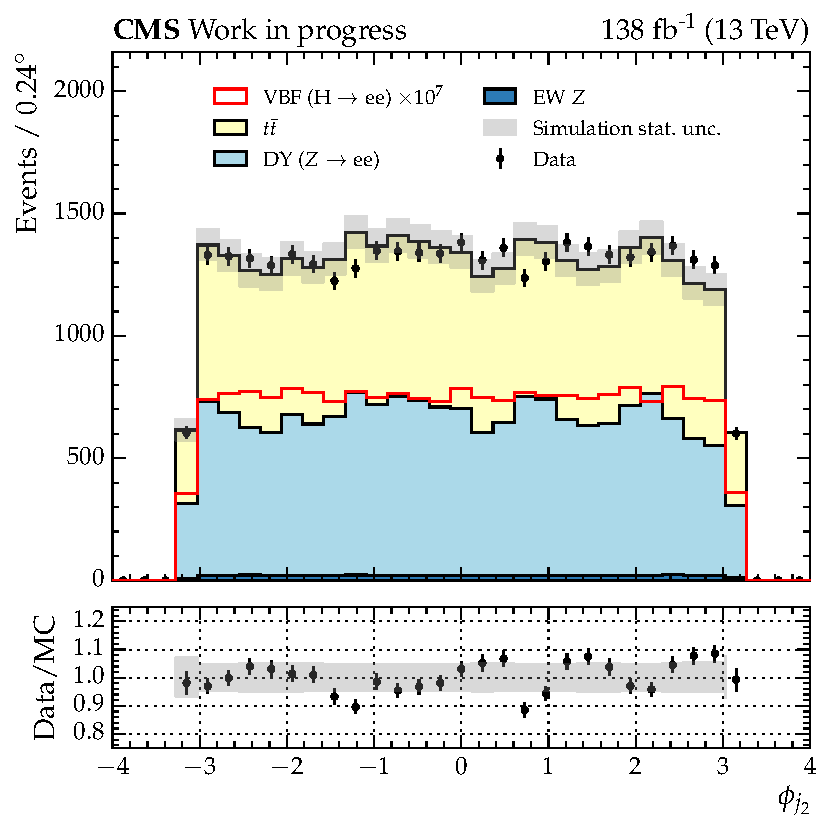
\includegraphics[width =0.33\linewidth]{Figures/Hee/VBF/dataMC/all_inputs/VBF_BDT_subleadJetPhi.pdf}
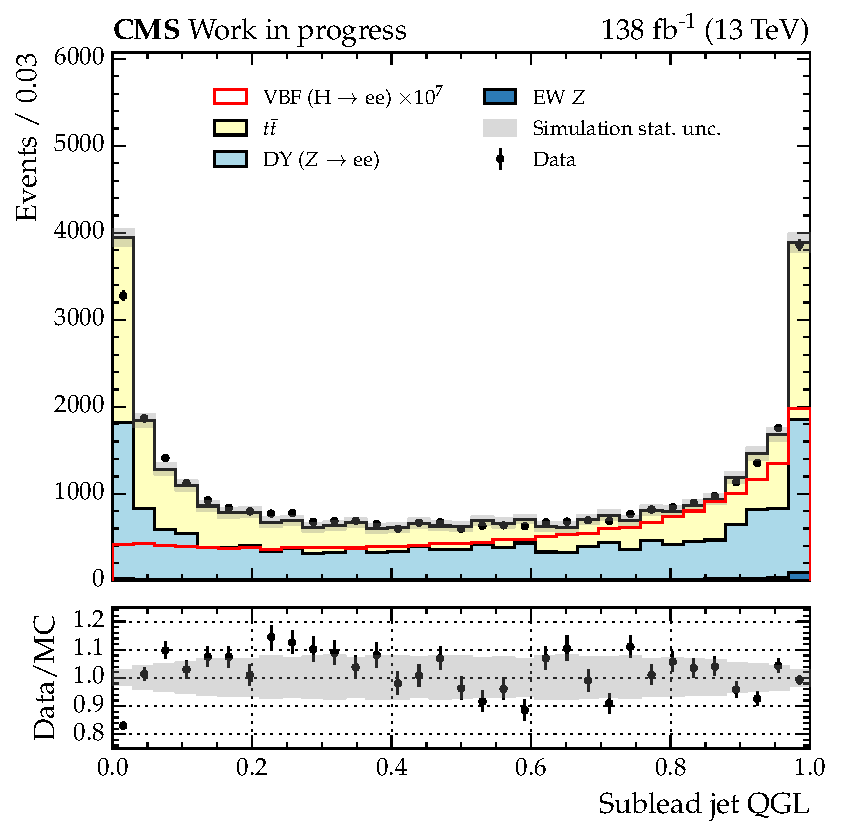
\includegraphics[width =0.33\linewidth]{Figures/Hee/VBF/dataMC/all_inputs/VBF_BDT_subleadJetQGL.pdf}\hfill%
\caption{Distributions for the input variables to the VBF BDT. The VBF signal is shown in red, with the overall normalisation scaled such that it is visible. The simulated background processes (bold face) are stacked for comparison with data (black points). Good agreement is observed between data and simulation, with respect to the statistical uncertainty (grey band).} 
\end{figure}

\begin{figure}[htbp!]
\centering
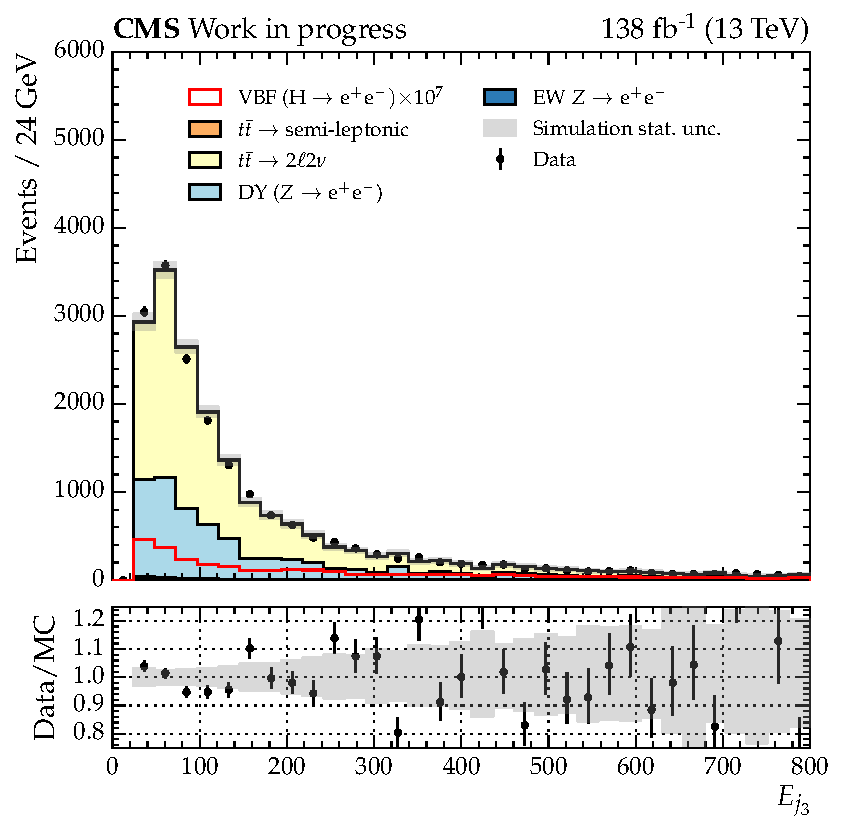
\includegraphics[width =0.33\linewidth]{Figures/Hee/VBF/dataMC/all_inputs/VBF_BDT_subsubleadJetEn.pdf}\hfill%
\includegraphics[width =0.33\linewidth]{Figures/Hee/VBF/dataMC/all_inputs/VBF_BDT_subsubleadJetPt.pdf}\hfill%
\includegraphics[width =0.33\linewidth]{Figures/Hee/VBF/dataMC/all_inputs/VBF_BDT_subsubleadJetEta.pdf}\hfill%
\includegraphics[width =0.33\linewidth]{Figures/Hee/VBF/dataMC/all_inputs/VBF_BDT_subsubleadJetPhi.pdf}
\includegraphics[width =0.33\linewidth]{Figures/Hee/VBF/dataMC/all_inputs/VBF_BDT_subsubleadJetQGL.pdf}\hfill%
\caption{Distributions for the input variables to the VBF BDT. The VBF signal is shown in red, with the overall normalisation scaled such that it is visible. The simulated background processes (bold face) are stacked for comparison with data (black points). Good agreement is observed between data and simulation, with respect to the statistical uncertainty (grey band).}
\label{fig:VBF_inputs_last}
\end{figure}